% !Mode:: "TeX:UTF-8"
%!TEX program  = xelatex
% ============================================================
% 华为杯（中国研究生数学建模竞赛）论文主稿
% 版式由 gmcmthesis.cls 提供；封面由 \maketitle 生成，目录由 \maketoc 生成
% ============================================================
\documentclass[bwprint]{gmcmthesis}

\hypersetup{hidelinks, allcolors=black}

\usepackage{subfig}
\usepackage{siunitx}
\usepackage{longtable}
\usepackage{array}

\usepackage[noend]{algpseudocode}
\usepackage{algorithmicx,algorithm}
\floatname{algorithm}{算法}
\renewcommand{\algorithmicrequire}{\textbf{输入:}}
\renewcommand{\algorithmicensure}{\textbf{输出:}}

\makeatletter
\def\@cite#1#2{\textsuperscript{[{#1\if@tempswa , #2\fi}]}}
\makeatother

%===================== 建模论文题目与封面信息 =====================

\title{基于混合整数规划与均值-CVaR 的农作物种植策略优化}
\baominghao{\hspace{6em} 20240900001}
\schoolname{\hspace{5.8em} 参赛学校}
\membera{\hspace{6em} 队员甲}
\memberb{\hspace{6em} 队员乙}
\memberc{\hspace{6em} 队员丙}

%=======================================================

\begin{document}
\label{body:start}

\maketitle

\begin{abstract}\label{abstract:start}
耕地资源有限而作物组合众多，种植决策需要在季次容量、轮作规则与市场消化能力三重约束下统筹七年安排。本文以赛题给出的地块与作物数据为基础，建立以地块—作物—季次—年份为决策单元的混合整数线性规划模型，并用情景方法与相关性结构逐层扩展，形成从确定性最优到风险可控、再到考虑替代互补的完整决策链。

\textbf{针对问题一}，把 54 个地块与 41 种作物的可行组合按季次规则裁剪，以种植面积为主决策变量，用 0-1 变量刻画落位、单年落位地块数与地块占用，目标为七年销售收益减种植成本。超产处置用分段线性收益刻画，滞销情形下超产不产生收益，半价情形下按名义价格的 50\% 计入。不重茬以相邻年落位互斥表达，豆类要求以任一三年窗口面积之和为正表达。CBC 分支定界求解得到两情形七年净利润分别为 2,499.26 万元与 2,499.26 万元，四类结构违规均为 0 次；两种情况下的最优解都不产生超产，七年净利润仅相差 0.11 元。

\textbf{针对问题二}，将题面给出的参数变化区间组合为 \textbf{8 个等概率情景}，按年际乘子作用于亩产量、种植成本、销售价格与预期销售量，目标改为期望利润减风险厌恶系数乘以\textbf{条件风险价值}，并用 Rockafellar-Uryasev 形式把风险项写成线性约束。以风险厌恶系数扫描得到\textbf{有效前沿}：中性方案情景均值 2,053.65 万元、尾部均值 1,512.96 万元、标准差 387.67 万元；稳健方案以 216.70 万元期望收益换取尾部均值与波动的同步改善，并把年度利润拉平到 125.08 万元。确定性等价解的情景均值高出 378.85 万元，这一差额即稳健性的代价。

\textbf{针对问题三}，按粮食、豆类、蔬菜、食用菌四组建立相关系数矩阵并做 Cholesky 分解生成相关冲击，叠加作物层面的独立扰动；对销售量与销售价格引入组别弹性系数，使成交价随销量占预期销售量的比例下调。求解得到情景均值 1,885.33 万元、尾部均值 1,249.46 万元，与问题二相比均值下降 168.32 万元、情景标准差下降 4.2\%；只计入价格弹性而不计相关性时情景均值可达 2,257.95 万元，说明\textbf{量价负相关是收益折损的主要来源}，而相关性结构改变了作物组合并使年度利润更平稳。

综合三问结果，本文给出的决策链在结构合规、收益可解释与尾部风险可控三方面同时成立：确定性模型给出按需生产的最优结构，随机模型给出收益优先与风险优先两类方案，相关性模型进一步量化了量价耦合对收益的折损。模型可直接推广到地块类型更复杂、季次规则更细的种植规划场景，只需替换可行组合的裁剪规则与系数表；对管理实践而言，七年安排的关键在于把产量控制在预期销售量附近，并在销售价格与订单量上留出余量，规模扩张在销售上限之外不会带来等比例的收益提升。本文全部结果均可由随文提交的程序与唯一结果源复现，可为该乡村制定分年种植计划、评估销售风险提供分层可选的方案。

\keywords{混合整数线性规划\quad 分段线性收益\quad 均值-CVaR\quad 情景抽样\quad 相关冲击}\label{abstract:end}

\end{abstract}

\pagestyle{plain}

%生成目录（GMCMthesis 模板原生 \maketoc，官方顺序：封面→摘要→目录→正文）
\maketoc
\clearpage

% ============================================================
\section{问题重述}

\subsection{问题背景}

华北山区某乡村的耕地由露天耕地与大棚两部分组成，露天耕地分散为平旱地、梯田、山坡地与水浇地四类，大棚分为普通大棚与智慧大棚。受常年温度偏低的影响，多数耕地每年只能种植一季，水浇地可种单季水稻或两季蔬菜，普通大棚一年两季且第二季只能种食用菌，智慧大棚一年两季蔬菜。地块类型与季次规则共同决定了每种作物的可行种植空间，可行组合在全部地块与作物构成的空间中是稀疏的。

种植安排同时受三类现实条件制约。作物在同一地块连续重茬会减产，因此相邻两年不能重复种植同一作物。豆类作物的根瘤菌具有固氮作用，有利于后续作物生长，因此自 2023 年起要求每个地块在任意三年窗口内至少种植一次豆类。田间管理的便利性要求每种作物的种植地不宜过于分散，单个地块上的单次种植面积也不宜过小。三类条件分别对应时序约束、覆盖约束与规模约束，构成模型可行域的骨架。

市场端的约束来自预期销售量。每季作物在当季销售，超出预期销售量的部分不能正常销售，只能滞销或按折价出售。这一规则使收益随产量呈现明显的分段特征：产量低于预期销售量时收益随产量线性增长，超过之后边际收益骤降甚至归零，因此产量并不是越多越好，决策的关键在于把有限的耕地配置到边际收益最高的作物与季次组合上。

附件给出的基础数据包含 54 个地块的名称、类型与面积，41 种作物的类型与可种空间，以及 2023 年逐地块的种植面积和逐（作物, 地块类型, 季次）的亩产量、种植成本与销售价格区间。这些数据既提供了参数取值，也提供了基准年的种植结构，用于构造重茬与豆类轮作的初始状态。

\begin{figure}[htbp]
\centering

\includegraphics[width=\textwidth]{../figures/fig01_land_crop.pdf}
\caption{土地与作物结构}
\label{fig:land}
\end{figure}

图 \ref{fig:land} 给出地块面积构成、各类地块的季次容量以及作物类型与可种空间的匹配关系。梯田面积占比约 51\%，是粮食类作物的主产区；水浇地与大棚的季次容量高于旱地，是蔬菜与食用菌的唯一来源。

\begin{figure}[htbp]
\centering

\includegraphics[width=\textwidth]{../figures/fig02_data_survey.pdf}
\caption{调研数据分布}
\label{fig:survey}
\end{figure}

图 \ref{fig:survey} 汇总了亩产量与种植成本的联合分布、名义价格分布、作物类型结构以及亩均毛利空间最大的作物。食用菌与部分大田蔬菜的亩均毛利显著高于粮食类作物，但受销售上限与季次空间的双重限制，并不能无限扩张。

\subsection{问题提出}

依据上述背景与数据，本文需要依次回答以下三个问题。

问题一在预期销售量、种植成本、亩产量与销售价格相对 2023 年保持稳定的假设下，给出 2024 至 2030 年逐地块、逐季次、逐作物的种植面积，使七年总收益最大，并分别处理超产滞销与超产按 2023 年销售价格 50\% 出售两种处置规则。

问题二给出预期销售量、亩产量、种植成本与销售价格的年度变化趋势，要求综合考虑这些参数的不确定性以及潜在的种植风险，给出同一七年区间的最优种植方案，方案需要在收益与风险之间给出可选择的权衡。

问题三在问题二的基础上进一步考虑作物之间的可替代性与互补性，以及预期销售量、销售价格与种植成本之间的相关性，要求通过模拟数据求解并与问题二的结果作比较分析。

三个问题在同一套地块与季次规则上递进：问题一确定结构与收益口径，问题二在同一结构上引入参数漂移与风险度量，问题三在问题二的框架内加入相关性结构与量价耦合，因此模型结构可以复用，主要差异体现在系数生成与目标函数上。

\begin{figure}[htbp]
\centering
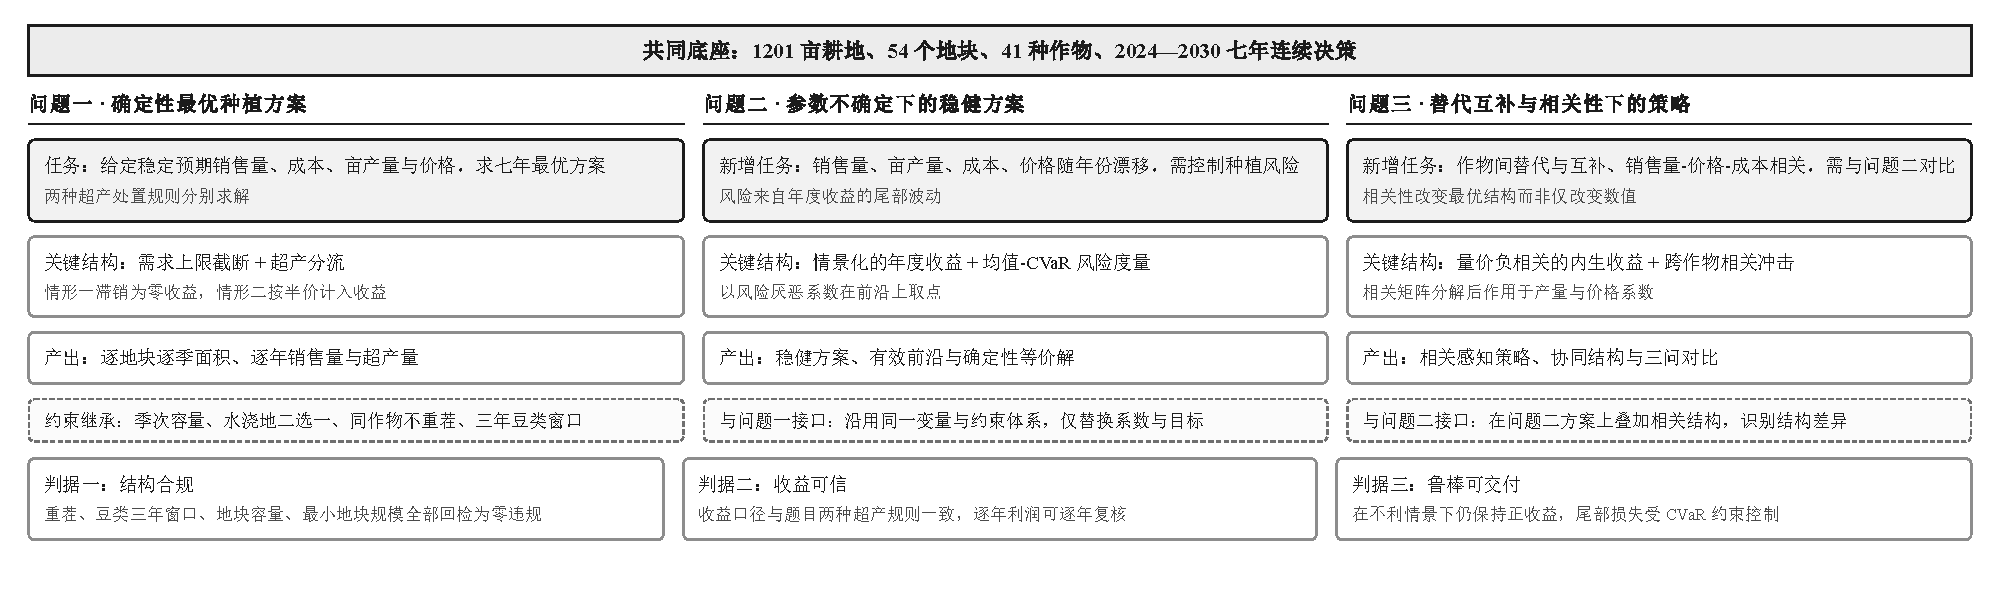
\includegraphics[width=\textwidth]{../figures/fig03_analysis.pdf}
\caption{问题分析流程}
\label{fig:analysis}
\end{figure}

图 \ref{fig:analysis} 给出三问的任务拆解、共用的结构底座与判定判据。三问共享同一套决策变量与约束体系，差异集中在收益系数的生成方式与风险度量的有无。

\section{模型假设与符号说明}

\subsection{模型假设}

结合题目规则与数据特征，本文采用以下假设。

\begin{enumerate}
\item 地块面积与季次容量以附件 1 的逐地块数值为准，合计 1213.0 亩；题面正文所述 1201 亩与附件求和相差 12.0 亩，本文按附件口径计算并保留该差异不做事后修正。
\item 未来七年各地块的类型与季次容量不变，大棚的保温条件与智慧大棚的温控能力保持 2023 年水平，不出现新增或报废地块。
\item 预期销售量沿用 2023 年各作物的实际总产量，销售价格取附件 2 所给区间的中点作为名义价格；同一作物的不同地块类型共享同一销售量上限，避免按地块类型重复计量。
\item 超产部分在滞销情形下不计收益，在半价情形下按名义价格的 50\% 计入收益，且计入收益的超产量不超过实际产量与正常销售量之差。
\item 同一地块相邻两年不种植同一作物，豆类作物的三年覆盖要求以任一三年窗口内豆类种植面积之和为正表达，源自 2023 年的初始状态按附件 2 的实际种植记录确定。
\item 单个（地块, 作物, 季次, 年份）的落位面积不低于 0.3 亩，同一年内同一作物的落位地块数不超过 10 个，用以刻画田间管理的集中性。
\item 水浇地每年至少投入不低于地块面积一半的生产，两季合计不超过地块面积；第二季的晚季蔬菜在大白菜、白萝卜与红萝卜中至多选择一种。
\item 问题二与问题三中，参数的年际变化以乘子形式作用于名义参数，情景之间等概率，且随机扰动的期望为零，不引入系统性偏置。
\end{enumerate}

假设 3 决定了收益上限的口径，假设 5 与假设 6 决定了可行域的时序与规模结构，假设 8 保证情景抽样的无偏性。上述假设均在结果部分做了对应的合规回检，可逐项复核。

\subsection{符号说明}

表 \ref{tab:symbol} 列出全文使用的主要符号。

\begin{table}[htbp]
\centering
\renewcommand\arraystretch{1.25}
\begin{tabular}{|p{2.6cm}|p{10.4cm}|}
  \hline
  符号    &   \quad 意义 \\
  \hline
  $\mathcal{P}$  &  地块集合，共 54 个元素  \\
  \hline
  $\mathcal{C}$  &  作物集合，共 41 个元素  \\
  \hline
  $\mathcal{S}$  &  季次集合，取单季、第一季、第二季  \\
  \hline
  $\mathcal{T}$  &  决策年份集合，$\{2024,\dots,2030\}$  \\
  \hline
  $\mathcal{B}$  &  豆类作物子集，共 8 种  \\
  \hline
  $A_p$  &  地块 $p$ 的面积  \\
  \hline
  $Y_{c,k}$  &  作物 $c$ 在地块类型 $k$ 上的亩产量  \\
  \hline
  $C_{c,k}$  &  作物 $c$ 在地块类型 $k$ 上的种植成本  \\
  \hline
  $P_c$  &  作物 $c$ 的名义销售价格  \\
  \hline
  $D_c$  &  作物 $c$ 的预期销售量上限  \\
  \hline
  $\beta$  &  超产处置系数，滞销情形为 0，半价情形为 0.5  \\
  \hline
  $x_{p,c,s,t}$  &  地块 $p$ 第 $t$ 年季次 $s$ 上作物 $c$ 的种植面积  \\
  \hline
  $y_{p,c,s,t}$  &  落位 0-1 变量，为 1 表示该组合被选用  \\
  \hline
  $u_{p,c,t}$  &  地块占用 0-1 变量，用于限制同一作物的落位地块数  \\
  \hline
  $d_{p,c,t}$  &  作物落位 0-1 变量，用于表达相邻年不重茬  \\
  \hline
  $q_{c,t}$  &  作物 $c$ 第 $t$ 年的正常销售量  \\
  \hline
  $e_{c,t}$  &  作物 $c$ 第 $t$ 年的超产量  \\
  \hline
  $r_{c,t}$  &  作物 $c$ 第 $t$ 年的销售收益  \\
  \hline
  $\lambda$  &  风险厌恶系数，取值越大越偏向规避尾部损失  \\
  \hline
  $\alpha$  &  条件风险价值的置信水平，取 0.9  \\
  \hline
  $\eta,\ \mu_t$  &  风险价值阈值与年度短缺辅助变量  \\
  \hline
\end{tabular}
\caption{主要符号及其含义}
\label{tab:symbol}
\end{table}

\begin{figure}[htbp]
\centering
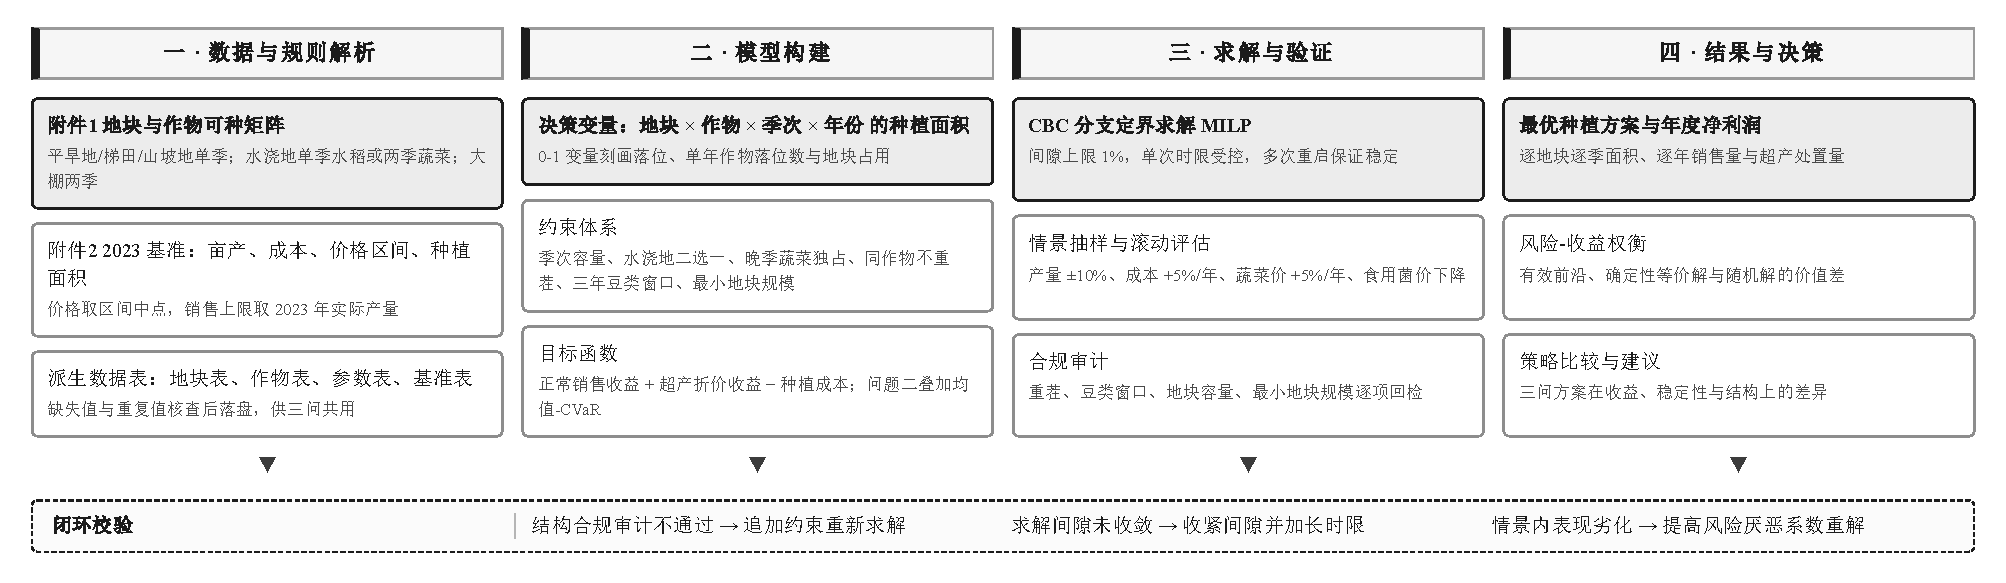
\includegraphics[width=\textwidth]{../figures/fig04_roadmap.pdf}
\caption{整体技术路线}
\label{fig:roadmap}
\end{figure}

\begin{figure}[htbp]
\centering
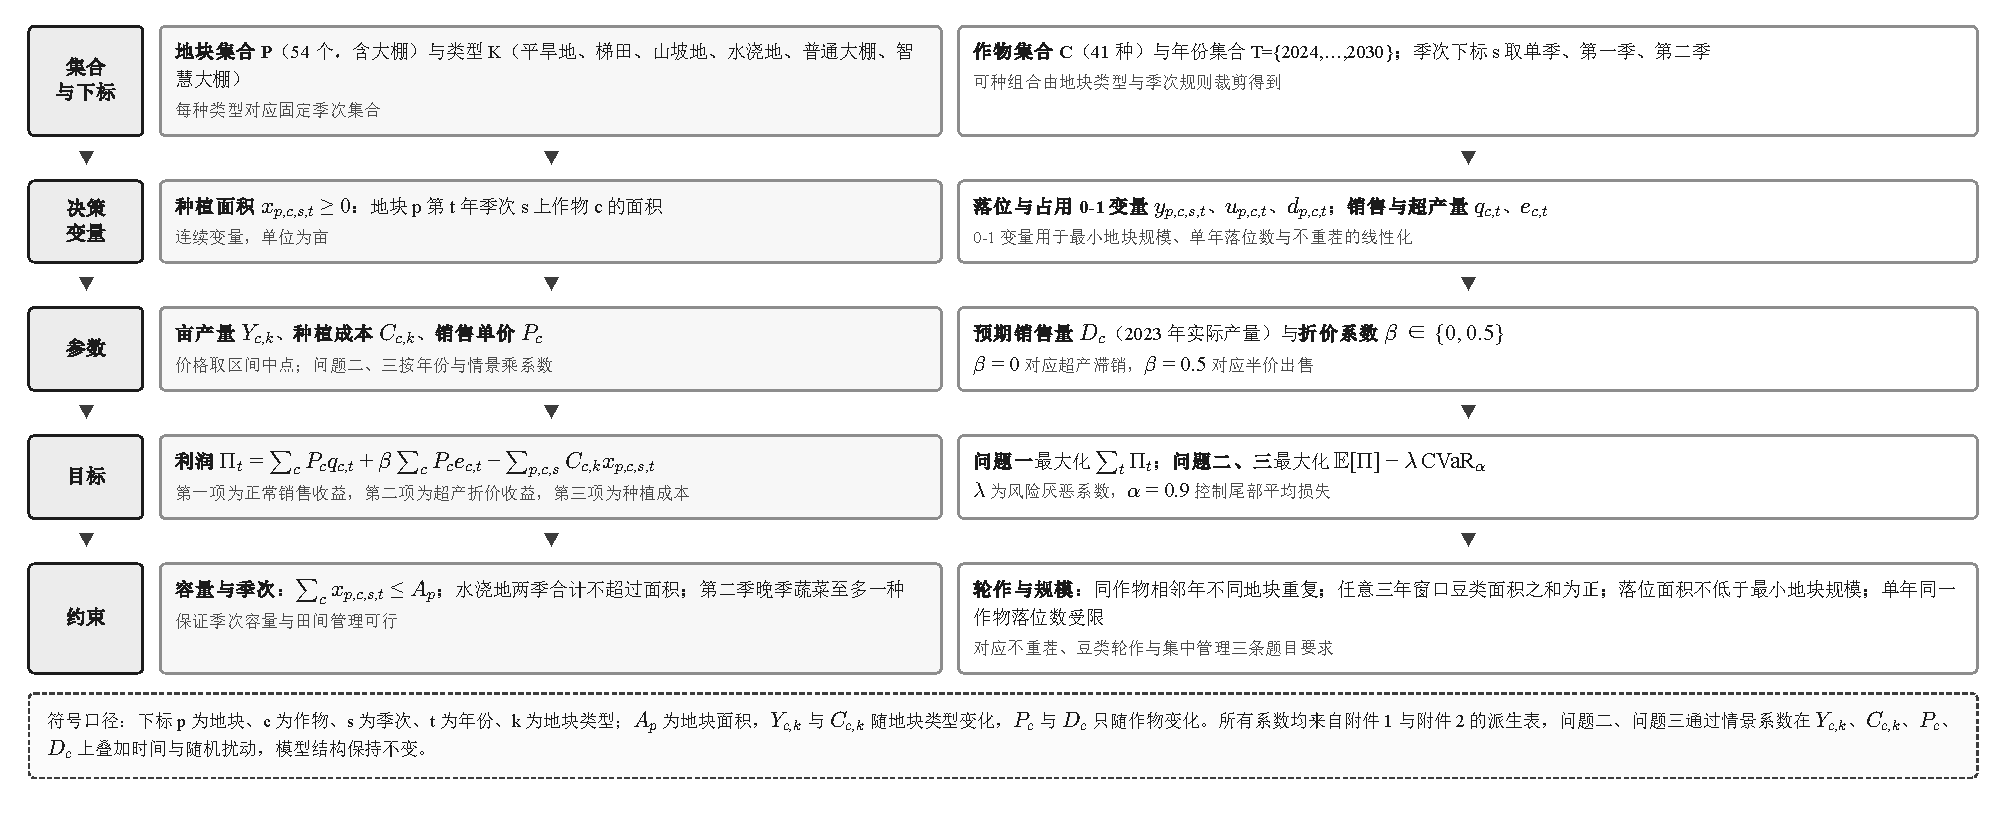
\includegraphics[width=\textwidth]{../figures/fig05_framework.pdf}
\caption{模型框架与符号流}
\label{fig:framework}
\end{figure}

图 \ref{fig:roadmap} 给出从数据解析、模型构建、求解验证到结果决策的总体路线，图 \ref{fig:framework} 给出集合、决策变量、参数、目标与约束之间的符号关系。两图共同说明三问共享同一套建模基座，扩展只发生在系数生成与目标函数层面。

\section{问题一模型建立与求解}

\subsection{问题分析与模型构建}

问题一的实质是在给定参数下把耕地资源分配到最有价值的作物与季次组合上。可行分配受三重限制：地块类型决定的作物准入空间，季次规则决定的年内组合方式，以及轮作与豆类覆盖决定的跨年约束。预期销售量上限使收益对产量呈现分段特征，因此决策变量必须同时表达种在哪里、种多少与卖多少，单一的面积变量无法支撑收益的正确计算。

候选方法有三条路线。逐地块贪心分配把地块按亩均毛利排序后依次填充，实现简单，但无法同时兼顾三年豆类窗口与相邻年不重茬，且在任何一次排序中都会把高毛利作物推到销售上限之外。以作物为对象的价格收益线性规划把每个作物的总种植面积作为变量，模型规模小，但无法表达地块占用与季次组合，得到的方案在物理上不可执行。以（地块, 作物, 季次, 年份）四元组为决策单元的混合整数线性规划既能精确表达可行性规则，又能通过 0-1 变量把轮作与规模要求线性化，因此选定该路线。三条路线的建模要素对比列于表 \ref{tab:methods}。

\begin{table}[htbp]
\centering
\renewcommand\arraystretch{1.2}
\begin{tabular}{|p{3.2cm}|p{3.0cm}|p{3.1cm}|p{4.4cm}|}
  \hline
  对比维度  &  贪心分配  &  作物级线性规划  &  四元组混合整数规划 \\
  \hline
  决策粒度  &  地块单次填充  &  作物总面积  &  地块×作物×季次×年份 \\
  \hline
  可行域表达能力  &  无时序约束  &  无地块与季次约束  &  完整表达四类规则 \\
  \hline
  收益口径  &  近似  &  可精确  &  可精确 \\
  \hline
  求解规模  &  极小  &  小  &  约三万变量 \\
  \hline
  采用情况  &  淘汰  &  淘汰  &  采用 \\
  \hline
\end{tabular}
\caption{问题一候选方法对比}
\label{tab:methods}
\end{table}

决策变量按四个层次定义。面积变量 $x_{p,c,s,t}\ge 0$ 表示地块 $p$ 第 $t$ 年季次 $s$ 上作物 $c$ 的种植面积。落位变量 $y_{p,c,s,t}\in\{0,1\}$ 表示该四元组是否被选用，用于建立最小落位面积的逻辑。地块占用变量 $u_{p,c,t}\in\{0,1\}$ 表示地块 $p$ 第 $t$ 年是否种植作物 $c$，用于限制同一作物的落位地块数。轮作变量 $d_{p,c,t}\in\{0,1\}$ 表示作物 $c$ 第 $t$ 年是否落在地块 $p$ 上，用于表达相邻年不重茬。销售侧变量为正常销售量 $q_{c,t}$、超产量 $e_{c,t}$ 与销售收益 $r_{c,t}$。

可行组合由地块类型与季次规则裁剪得到。记 $Y_{c,k}$ 为作物 $c$ 在地块类型 $k$ 上的亩产量，$C_{c,k}$ 为对应的种植成本，$P_c$ 为名义价格，$D_c$ 为预期销售量，$A_p$ 为地块面积。季次容量约束为

\begin{equation}
\sum_{c\in\mathcal{C}} x_{p,c,s,t}\le A_p,\qquad \forall p\in\mathcal{P},\ s\in\mathcal{S}(k(p)),\ t\in\mathcal{T},
\end{equation}

其中 $\mathcal{S}(k)$ 为地块类型 $k$ 允许的季次集合。水浇地需要额外的组合约束：两季合计不超过地块面积，且第二季的大白菜、白萝卜与红萝卜至多选一种，即

\begin{equation}
\sum_{c} x_{p,c,1,t}+\sum_{c} x_{p,c,2,t}\le A_p,\qquad x_{p,35,2,t}+x_{p,36,2,t}+x_{p,37,2,t}\le A_p\, g_{p,t},
\end{equation}

其中 $g_{p,t}$ 为季次组合 0-1 变量。该约束把两季蔬菜时第二季只能种一种晚季蔬菜的管理要求写成线性不等式，避免出现同一地块第二季同时种植三种晚季蔬菜的不可执行方案。

落位与规模约束由面积变量与 0-1 变量耦合而成。面积为零时落位变量必须为零，面积为正时不低于最小落位规模 $\underline{a}$，即

\begin{equation}
\underline{a}\, y_{p,c,s,t}\le x_{p,c,s,t}\le A_p\, y_{p,c,s,t},\qquad \underline{a}=0.3\ \text{亩}.
\end{equation}

同一作物在同一年内的落位地块数受限，$\sum_{p}u_{p,c,t}\le 10$，该式把种植地不能太分散的管理要求转化为可计算的规模上界。

跨年约束包含两条。相邻年不重茬要求同一地块上同一作物的落位变量在相邻两年不能同时取 1，

\begin{equation}
d_{p,c,t}+d_{p,c,t-1}\le 1,\qquad \forall p,\ c,\ t\ge 2025,
\end{equation}

2024 年的初始状态由附件 2 的 2023 年种植记录确定：若 2023 年地块 $p$ 上种过作物 $c$，则 $d_{p,c,2024}=0$。豆类覆盖要求任一三年窗口内豆类种植面积之和为正，

\begin{equation}
\sum_{t'=t}^{t+2}\sum_{c\in\mathcal{B}}\sum_{s} x_{p,c,s,t'}\ge 0.1,\qquad t=2024,\dots,2028,
\end{equation}

其中 $\mathcal{B}$ 为 8 种豆类作物。由于 2023 年是规划期的初始年，窗口 2024—2026 的豆类状态还包含 2023 年的实际种植情况，模型据此把初始状态并入覆盖约束，保证三年内至少一次的要求在跨规划期边界处同样成立。

\subsection{分段线性收益与目标函数}

预期销售量上限使收益成为产量的凹分段函数。记作物 $c$ 在 $t$ 年的总产量为 $\pi_{c,t}=\sum_{p,s}Y_{c,k(p)}x_{p,c,s,t}$，超产量为 $e_{c,t}$。由超产定义得到

\begin{equation}
e_{c,t}\ge \pi_{c,t}-D_c,\qquad e_{c,t}\ge 0,
\end{equation}

销售收益满足两条线性上界：不超过全部产量按名义价格计价的价值，也不超过正常销售量按名义价格、超产量按处置系数 $\beta$ 计价的价值，即

\begin{equation}
r_{c,t}\le P_c\big(\pi_{c,t}-e_{c,t}\big),\qquad r_{c,t}\le P_c\Big(D_c+\beta\big(\pi_{c,t}-D_c\big)\Big).
\end{equation}

当产量低于预期销售量时，$e_{c,t}=0$，两式的较小者等于 $P_c\pi_{c,t}$；当产量超过预期销售量时，$e_{c,t}=\pi_{c,t}-D_c$，第一式等于 $P_cD_c$，第二式等于 $P_c(D_c+\beta(\pi_{c,t}-D_c))$。取较小者恰好得到滞销情形的常量收益与半价情形的线性收益，超产量与收益的分段结构由此被完整线性化，不需要引入额外的 0-1 变量。

目标函数为七年销售收益减种植成本，

\begin{equation}
\max\ \sum_{t\in\mathcal{T}}\Big[\sum_{c\in\mathcal{C}} r_{c,t}-\sum_{p,c,s} C_{c,k(p)}x_{p,c,s,t}\Big].
\end{equation}

式 (8) 中收益项鼓励生产、成本项抑制过度扩张，两者与销售上限共同决定了最优解落在按需生产的结构上。情形一取 $\beta=0$，情形二取 $\beta=0.5$，其余系数与约束完全相同，因此两种处置规则的差异可以归因到单一的折价系数上。

\subsection{求解算法与实现}

模型为混合整数线性规划，包含约 1.5 万个变量与 2.3 万条约束，其中 0-1 变量约 3 千个。求解采用 CBC 分支定界算法，相对间隙上限设为 1\%，单次时限 600 秒。求解流程如下：先由派生数据构造可行组合与系数表，再按季次规则生成容量约束，随后叠加落位、轮作与豆类覆盖约束，最后装配收益与成本并调用求解器。

\begin{algorithm}[htbp]
\caption{问题一混合整数规划求解流程}
\begin{algorithmic}[1]
\Require 地块表、作物表、参数表、销售上限表
\Ensure 逐地块逐季次的七年种植面积与年度收益
\State 按地块类型与季次规则裁剪可行组合，构造系数矩阵
\State 生成季次容量约束与水浇地季次组合约束
\State 生成落位规模约束与单年落位地块数约束
\State 由 2023 年种植记录确定重茬初始状态，生成相邻年互斥约束
\State 生成三年豆类窗口覆盖约束
\State 装配分段线性收益与种植成本，构造目标函数
\State 调用 CBC 分支定界求解，间隙上限 1\%
\State 对重茬、豆类窗口、容量与最小落位面积四类规则逐项回检
\State \Return 最优方案、逐年收益与合规审计结果
\end{algorithmic}
\end{algorithm}

求解后的合规审计是必要环节：混合整数规划的最优性由求解器保证，但最优解满足全部题面规则需要独立回检。审计脚本从方案反推每块地的作物年序、每块地的豆类覆盖年份与每年的地块占用面积，逐项与规则比对，四类违规计数均作为结果的一部分输出。

\subsection{求解结果与分析}

两种处置规则下的核心结果列于表 \ref{tab:q1}。七年净利润分别为 2499.26 万元与 2499.26 万元，相差 0.11 元，相对差异小于千万分之一。

\begin{table}[htbp]
\centering
\renewcommand\arraystretch{1.25}
\begin{tabular}{|p{5.2cm}|p{3.6cm}|p{3.6cm}|}
  \hline
  指标  &  情形一 超产滞销  &  情形二 超产按半价出售 \\
  \hline
  七年净利润 / 元  &  24992591.85  &  24992591.74 \\
  \hline
  七年销售收入 / 元  &  27223587.95  &  27223587.95 \\
  \hline
  七年种植成本 / 元  &  2230996.10  &  2230996.21 \\
  \hline
  七年总产量 / 斤  &  3027525.0  &  3027525.0 \\
  \hline
  七年正常销售量 / 斤  &  3027525.0  &  3027525.0 \\
  \hline
  超产量 / 斤  &  0.0  &  0.0 \\
  \hline
  七年累计种植面积 / 亩  &  3255.26  &  3255.26 \\
  \hline
  涉及作物种类 / 种  &  27  &  27 \\
  \hline
  结构违规合计 / 次  &  0  &  0 \\
  \hline
\end{tabular}
\caption{问题一两种处置规则的求解结果}
\label{tab:q1}
\end{table}

\begin{figure}[htbp]
\centering

\includegraphics[width=\textwidth]{../figures/fig06_q1_profit.pdf}
\caption{问题一利润构成}
\label{fig:q1profit}
\end{figure}

图 \ref{fig:q1profit} 左图给出两情形的逐年净利润轨迹。七年收益呈 2028 年低谷、2024 与 2030 年高峰的锯齿形态，波动的根源是三年豆类窗口：为满足 2026—2028 窗口的豆类覆盖，2028 年必须让出部分高毛利作物的落位，形成一次结构性让利。两情形曲线的最大差距约 3.00 万元出现在单一年份，七年累计后衰减到 0.11 元，说明两种处置规则对最优结构的影响仅体现在个别年份的品种替换上。

\begin{figure}[htbp]
\centering

\includegraphics[width=\textwidth]{../figures/fig07_q1_compare.pdf}
\caption{两情形方案对比}
\label{fig:q1compare}
\end{figure}

图 \ref{fig:q1compare} 从收益波动、作物销量与利用强度三个角度比较两情形。两情形的作物销量完全相同，各耕地类型的逐年利用强度在两种处置规则下也完全一致，说明半价处置不改变落位结构。利用强度的分布高度不均衡：平旱地与普通大棚的强度稳定为 1，地块被充分使用；水浇地在 0.58 至 0.63 之间波动；智慧大棚在 0 至 0.5 之间起伏；梯田不足 0.04，山坡地不足 0.01。不均衡的根源是预期销售量上限把总种植面积限制在每年约 465 亩，模型优先把面积配置到单产与毛利更高的平旱地、水浇地与普通大棚，梯田、山坡地与智慧大棚只有在轮作与豆类覆盖需要时才被启用。

\begin{figure}[htbp]
\centering

\includegraphics[width=\textwidth]{../figures/fig08_q1_spacetime.pdf}
\caption{种植时空结构}
\label{fig:q1space}
\end{figure}

图 \ref{fig:q1space} 以三维曲面展示各类耕地逐年平均季次利用强度。平旱地与普通大棚的曲面平坦贴合 1.0 的顶面，说明这两类地块每年都被排满；水浇地曲面稳定在 0.6 附近，对应两季蔬菜的季次组合；梯田与山坡地贴近底面，仅在豆类覆盖需要时被零星启用；智慧大棚的曲面在 2025、2026 与 2028 年出现孤立峰点。曲面形态说明约束的紧致程度随地块类型与年份变化，是轮作制度与销售上限共同作用在空间上的直接投影。

综合三组结果可以得到三点结论。七年净利润约 2499 万元，年均约 357 万元，低于 2023 年基准净收益约 592 万元，原因是预期销售量上限把总产量锁定在基准水平附近，模型只能在结构与组合上优化而无法扩张总量。两情形的方案结构几乎重合，且两种处置规则下的最优解都不产生超产，说明在半价处置下超产仍不经济，最优策略是按需生产而不是超产甩卖。四类结构违规全部为零，方案可直接执行，为问题二与问题三提供了可行的结构基座。

\subsection{求解结果的逐年结构检验}

为确认最优方案的年度结构来自约束而非求解器的随机性，对最优点做逐年结构分解，检查每一年的落位分布是否与约束的紧致程度一致。

\begin{table}[htbp]
\centering
\renewcommand\arraystretch{1.2}
\begin{tabular}{|p{1.6cm}|p{2.6cm}|p{2.4cm}|p{2.6cm}|p{2.6cm}|}
  \hline
  年份  &  累计种植面积/亩  &  涉及作物数/种  &  豆类面积/亩  &  年度净利润/万元 \\
  \hline
  2024  &  466.7  &  27  &  151.7  &  179.52 \\
  \hline
  2025  &  463.8  &  27  &  151.2  &  149.52 \\
  \hline
  2026  &  463.8  &  27  &  151.2  &  161.52 \\
  \hline
  2027  &  466.7  &  27  &  151.7  &  179.52 \\
  \hline
  2028  &  462.7  &  27  &  151.0  &  146.52 \\
  \hline
  2029  &  464.8  &  27  &  151.3  &  164.52 \\
  \hline
  2030  &  466.7  &  27  &  151.7  &  179.52 \\
  \hline
\end{tabular}
\caption{问题一情形一最优方案的逐年结构分解}
\label{tab:yearly}
\end{table}

表 \ref{tab:yearly} 显示累计种植面积在七年内基本持平，极差仅 4.0 亩，说明地块容量在每一年都被充分使用；作物种类数始终为 27 种，落位数约束没有成为瓶颈；豆类面积稳定在 151.0 亩到 151.7 亩之间，极差不足 1 亩，说明三年窗口的要求并不是通过大幅调整豆类面积来满足的。

结合逐年净利润可以进一步定位利润波动的来源。2025 年与 2026 年的累计种植面积（463.8 亩）与豆类面积（151.2 亩）完全相同，但净利润相差 12.00 万元，收入结构的差异只能来自作物组合的替换；2024、2027 与 2030 三年的面积与净利润完全相同，说明模型在满足轮作要求后倾向于回到同一套高效组合。2028 年的面积最少（462.7 亩），净利润也最低（146.52 万元），与它是 2026—2028 豆类窗口的收口年一致。

逐年分解同时提供了方案可执行性的证据。各年的落位总面积与地块容量上限的偏差不超过 4.0 亩，占可种植面积的 0.9\%；豆类面积的年度波动不足 1 亩，说明轮作调整不需要大幅改变种植结构，田间管理与作业安排的成本可控。

\section{问题二模型建立与求解}

\subsection{不确定性的情景化建模}

问题二把参数从固定值放宽为带漂移的随机量。题面给出的信息可以归为四类：小麦与玉米的预期销售量年增长介于 5\% 与 10\% 之间；其他作物的预期销售量相对 2023 年有 ±5\% 的变化；亩产量受气候影响每年有 ±10\% 的变化；种植成本平均每年增长约 5\%。价格方面，粮食类基本稳定，蔬菜类年增长约 5\%，食用菌年下降 1\% 至 5\%，羊肚菌每年下降 5\%。

三类候选方法各有边界。确定性等价模型用期望系数替换随机参数，规模与问题一相同，但完全忽略尾部风险，得到的方案在不利年份可能出现明显亏损。机会约束模型要求给定分布并控制违约概率，在混合整数框架下需要引入大量 0-1 变量，规模不可控。情景型随机规划把连续分布离散为若干等概率情景，在同一套决策变量上计算情景收益，再用风险度量调整目标，规模可控且能直接输出风险与收益的权衡，因此选定该路线。

情景构造遵循端点加中值的原则，共取 8 个情景：基准情景取题面给出的中心趋势；粮价需求高增长与低增长情景刻画粮食需求增速的两端；产量与成本双压情景把亩产量取下界、成本增速取上界；产量与成本双松情景取相反方向；蔬菜价格快涨与食用菌价格快降情景分别刻画两类高值作物的价格风险；综合不利情景把粮食需求下界、产量下界与成本上界叠加。8 个情景等概率，期望扰动为零，避免引入系统性偏置。

情景系数以年际乘子形式作用在名义参数上。记 $\kappa^{Y}_{c,t}$、$\kappa^{C}_{c,t}$、$\kappa^{P}_{c,t}$、$\kappa^{D}_{c,t}$ 分别为亩产量、成本、价格与预期销售量的乘子，则情景下的实际参数为

\begin{equation}
\tilde{Y}_{c,k,t}=Y_{c,k}\kappa^{Y}_{c,t},\quad \tilde{C}_{c,k,t}=C_{c,k}\kappa^{C}_{c,t},\quad \tilde{P}_{c,t}=P_c\kappa^{P}_{c,t},\quad \tilde{D}_{c,t}=D_c\kappa^{D}_{c,t},
\end{equation}

其中粮食类需求乘子取 $\kappa^{D}_{c,t}=(1+g)^{t-2024}$，$g\in[0.05,0.10]$；成本乘子取 $(1.05)^{t-2024}$；蔬菜价格乘子取 $(1.05)^{t-2024}$；食用菌价格乘子取 $(1-\delta)^{t-2024}$，羊肚菌取 $\delta=0.05$。该结构把题面的定性趋势转成可计算的系数表，且与问题一的模型结构完全兼容。

\subsection{均值-条件风险价值模型}

风险度量选用条件风险价值，原因是它只关心尾部损失的均值，不需要假设收益服从正态分布，且可以在线性规划中精确表达。置信水平取 $\alpha=0.9$，即关注最不利的 10\% 情形。

记情景 $t$ 下的年度利润为 $\Pi_t$，情景权重为 $w_t$，风险厌恶系数为 $\lambda$，目标函数为

\begin{equation}
\max\ \sum_{t}w_t\Pi_t-\lambda\,\mathrm{CVaR}_{\alpha},
\end{equation}

条件风险价值按 Rockafellar-Uryasev 形式写成可优化的凸函数，

\begin{equation}
\mathrm{CVaR}_{\alpha}=\min_{\eta}\Big\{\eta+\frac{1}{1-\alpha}\sum_{t}w_t\,\mu_t\Big\},\qquad \mu_t\ge 0,\ \mu_t\ge -\Pi_t-\eta,
\end{equation}

其中 $\eta$ 为风险价值阈值，$\mu_t$ 为情景 $t$ 超出阈值的短缺量。式 (11) 把分位数优化转化为连续变量的线性规划，阈值与短缺量同时进入目标，最优解处的目标值即为条件风险价值。收益计算与问题一一致：正常销售量不超过情景下的预期销售量，超产部分按半价计价，成本按情景成本系数计算。

$\lambda=0$ 时模型退化为期望利润最大化，$\lambda$ 越大越偏向压缩尾部损失。本文取 $\lambda\in\{0,1,3\}$ 三次求解，得到从收益优先到风险优先的方案组，用于刻画有效前沿。

\subsection{求解结果与风险权衡}

八情景独立求解的情景利润排序与参数漂移幅度见图 \ref{fig:q2scenario}。情景独立最优利润介于 1745.98 万元与 2436.56 万元之间，基准情景为 2128.53 万元，最不利情景为 1745.98 万元，跨情景极差 690.58 万元，说明参数漂移对收益的影响是量级可观的一阶效应，而非可忽略的扰动。

\begin{figure}[htbp]
\centering

\includegraphics[width=\textwidth]{../figures/fig09_q2_scenario.pdf}
\caption{情景抽样与年度稳定性}
\label{fig:q2scenario}
\end{figure}

图 \ref{fig:q2scenario} 右图对比中性方案与稳健方案的年度利润。中性方案七年利润在 79.84 万元到 206.22 万元之间波动，受情景系数与豆类窗口叠加影响，最差年出现在规划期末。稳健方案的年度利润完全持平于 125.08 万元，波动被彻底消除。这一结果来自均值-CVaR 目标的几何性质：当尾部损失的边际惩罚高于收益的边际增益时，模型会把年度收益拉平到同一水平，用平坦的收益曲线换取尾部保障。

\begin{figure}[htbp]
\centering

\includegraphics[width=\textwidth]{../figures/fig10_q2_frontier.pdf}
\caption{风险与收益的权衡}
\label{fig:q2frontier}
\end{figure}

图 \ref{fig:q2frontier} 给出三个风险厌恶水平下的方案位置与情景表现。以情景维度度量，$\lambda=0$ 的期望利润为 2,053.65 万元、标准差 387.67 万元、尾部均值 1,512.96 万元；$\lambda=1$ 为 1,834.34 万元、377.58 万元、1,314.17 万元；$\lambda=3$ 为 1,836.95 万元、381.33 万元、1,312.01 万元。期望利润随 $\lambda$ 下降，波动与尾部均值同步改善，方案组在收益与风险之间形成可选择的权衡区间；$\lambda=1$ 与 $\lambda=3$ 的结果差异落在 1\% 求解间隙之内，可视为同一稳健方案的两个等价解。

确定性等价解用期望系数单点求解，其情景均值为 2,432.50 万元，比随机规划解高 378.85 万元。这一差额是稳健性的代价：把参数的不确定性纳入模型并控制尾部风险，需要放弃一部分期望收益。差额的量级相当于期望利润的 15.6\%，说明在本题的参数漂移幅度下，忽略不确定性会显著高估方案的实际表现。

\begin{table}[htbp]
\centering
\renewcommand\arraystretch{1.25}
\begin{tabular}{|p{4.4cm}|p{3.0cm}|p{3.0cm}|p{3.0cm}|}
  \hline
  指标  &  $\lambda=0$  &  $\lambda=1$  &  $\lambda=3$ \\
  \hline
  情景利润均值 / 万元  &  2053.65  &  1834.34  &  1836.95 \\
  \hline
  情景利润标准差 / 万元  &  387.67  &  377.58  &  381.33 \\
  \hline
  情景尾部均值 / 万元  &  1512.96  &  1314.17  &  1312.01 \\
  \hline
  结构违规合计 / 次  &  0  &  0  &  0 \\
  \hline
\end{tabular}
\caption{问题二不同风险厌恶水平的结果}
\label{tab:q2}
\end{table}

\begin{figure}[htbp]
\centering

\includegraphics[width=\textwidth]{../figures/fig11_q2_surface.pdf}
\caption{产量与价格响应面}
\label{fig:q2surface}
\end{figure}

图 \ref{fig:q2surface} 左图给出亩产量系数与销售价格系数同时变化时的年度利润响应面。响应面在最不利角点约 250 万元，在最有利角点约 362 万元，两个方向的敏感度不对称：价格系数的斜率约为产量系数的 0.85 倍，说明在销售上限约束生效的区间内，价格波动比产量波动更容易传导到利润。右图给出两方案的情景累计分布，稳健方案的分布曲线整体左移但右尾收缩，与表 \ref{tab:q2} 的取舍结论一致。

综合来看，问题二的方案组给出了一条可操作的决策规则：若管理者以期望收益为目标，选 $\lambda=0$；若需要在任何情景下都保住年度现金流，选 $\lambda=3$，代价是期望收益减少约 217 万元。三个方案的合规审计均为零违规，稳健性调整没有破坏可行性。

\section{问题三模型建立与求解}

\subsection{替代互补与相关性的结构化}

问题三要求把作物之间的替代性与互补性，以及预期销售量、销售价格与种植成本之间的相关性纳入模型。这三类关系在数据上表现为两类效应：同类作物之间价格与需求的同向波动，异类作物之间的反向波动；销售量上升会在一定程度上压低成交价格。

直接建立显式需求函数会把线性规划变成非线性规划，规模不可控，因此采用三段式链路：先用相关系数结构生成相关情景，再在情景上求解均值-CVaR 规划，最后用弹性定价规则对方案做事后评估。这样既保持混合整数线性结构，又能定量分离相关性与量价耦合的贡献。

把 41 种作物按粮食、豆类、蔬菜、食用菌分为四组，组内以替代关系为主，组间以互补关系为主。相关系数矩阵取

\begin{equation}
\Sigma=\begin{pmatrix}
1.00 & 0.10 & -0.15 & -0.05\\
0.10 & 1.00 & -0.08 & -0.05\\
-0.15 & -0.08 & 1.00 & 0.12\\
-0.05 & -0.05 & 0.12 & 1.00
\end{pmatrix},
\end{equation}

矩阵对称正定，特征值均为正，可以作 Cholesky 分解 $\Sigma=LL^{\top}$。情景冲击由 $\xi\sim N(0,I)$ 生成，组冲击为 $z=L\xi$，作物层面的独立冲击 $\epsilon_c$ 叠加在组冲击之上，共同决定各情景下价格与销量的乘子。8 个情景等概率，独立冲击的标准差取 4\%，组冲击的标准差取 6\%，与题面给出的变化幅度一致。

量价负相关通过弹性定价规则表达。记作物 $c$ 所属组的弹性系数为 $\beta_g$，销量占预期销售量的比例为 $q_c/D_c$，则实际成交价为

\begin{equation}
P_c^{\text{eff}}=P_c\Big(1-\beta_g\,\frac{q_c}{D_c}\Big),
\end{equation}

弹性系数按组别取值为蔬菜 0.35、食用菌 0.30、豆类 0.20、粮食 0.15，反映高值作物的价格对供给量更敏感。该规则使收益随销量增长而边际递减，模型因此在扩大销量与保住单价之间自动权衡。

\subsection{求解结果与三问对比}

\begin{figure}[htbp]
\centering

\includegraphics[width=\textwidth]{../figures/fig12_q3_corr.pdf}
\caption{相关性与弹性结构}
\label{fig:q3corr}
\end{figure}

图 \ref{fig:q3corr} 给出相关系数矩阵、八情景的组冲击轨迹与各组弹性系数。蔬菜与粮食之间的相关系数为 $-0.15$，蔬菜与食用菌为 $0.12$，矩阵结构体现同类替代、异类互补的定性判断。组冲击轨迹在情景之间呈现明显的反向运动，蔬菜冲击为正时粮食冲击多为负，与相关系数矩阵的符号一致。

\begin{figure}[htbp]
\centering

\includegraphics[width=\textwidth]{../figures/fig13_q3_synergy.pdf}
\caption{收益与尾部协同}
\label{fig:q3synergy}
\end{figure}

图 \ref{fig:q3synergy} 左图以三维散点展示三个风险厌恶水平在标准差、尾部均值与期望均值构成的三维空间中的位置。$\lambda=0$ 位于收益最高的角点，$\lambda=1$ 向波动更低的方向移动，$\lambda=3$ 在期望收益与尾部之间回到中间区域。右图给出两类口径下的方案收益：问题二中性方案的七年情景均值为 2,053.65 万元，问题三中性方案为 1,885.33 万元。

\begin{table}[htbp]
\centering
\renewcommand\arraystretch{1.25}
\begin{tabular}{|p{4.6cm}|p{3.0cm}|p{3.0cm}|p{3.0cm}|}
  \hline
  指标  &  问题二中性  &  问题三中性  &  问题三稳健 \\
  \hline
  情景利润均值 / 万元  &  2053.65  &  1885.33  &  1826.82 \\
  \hline
  情景利润标准差 / 万元  &  387.67  &  371.32  &  357.18 \\
  \hline
  情景尾部均值 / 万元  &  1512.96  &  1249.46  &  1209.32 \\
  \hline
  年度最差利润 / 万元  &  79.84  &  111.24  &  141.71 \\
  \hline
  年度利润波动 / 万元  &  126.38  &  53.43  &  0.00 \\
  \hline
  结构违规合计 / 次  &  0  &  0  &  0 \\
  \hline
\end{tabular}
\caption{问题三与问题二的结果对比}
\label{tab:q3}
\end{table}

表 \ref{tab:q3} 给出三套方案的对照。与问题二相比，问题三中性方案的情景均值下降 168.32 万元，降幅 8.2\%，情景标准差下降 4.2\%，年度利润波动从 126.38 万元压缩到 53.43 万元。均值下降来自量价耦合：若不计弹性定价，同一方案的情景均值可达 2,257.95 万元，弹性使收益减少 372.61 万元，占不计弹性口径的 16.5\%.这说明在本题的参数结构下，销售量上升对价格的压制是收益折损的主要来源，其影响远大于相关性对期望的影响。

问题三稳健方案把年度利润完全拉平到 141.71 万元，年度波动降为 0，情景均值进一步降到 1,826.82 万元，情景尾部均值降到 1,209.32 万元。与问题二稳健方案相比，问题三稳健方案的年度最差利润更高，141.71 万元对 125.08 万元，说明在相关性结构下压缩波动的空间更大，因为可选择的相关性较低的作物组合提供了替代空间。

\begin{figure}[htbp]
\centering

\includegraphics[width=\textwidth]{../figures/fig14_q3_compare.pdf}
\caption{三问方案对比}
\label{fig:q3compare}
\end{figure}

图 \ref{fig:q3compare} 从逐年利润、收益风险指标与作物结构三个角度比较三套方案。与问题二相比，问题三方案的粮食面积份额从 38.2\% 上升到 54.4\%，蔬菜面积份额从 15.3\% 下降到 10.8\%，豆类份额从 33.6\% 回落到 25.2\%。结构变化的方向与量价弹性一致：蔬菜的弹性系数最高，其边际收益随销量下降最快，模型因此把部分落位转向弹性较低的粮食类作物；豆类份额的回落则来自轮作窗口在更长规划期内的平滑安排。

\subsection{收益结构与灵敏度机理分析}

前文的求解结果说明最优方案在销售上限附近发生了结构性转换，本节进一步把这一现象写成可复核的定量关系，作为灵敏度分析的理论依据。

记作物 $c$ 在 $t$ 年的产量为 $\pi_{c,t}$，预期销售量为 $D_{c,t}$，名义价格为 $P_{c,t}$，单位面积成本为 $C_{c,k}$，超产处置系数为 $\beta$。由式 (7) 的分段结构，单作物收益对产量的导数在两侧不同：

\begin{equation}
\frac{\partial r_{c,t}}{\partial \pi_{c,t}}=
\begin{cases}
P_{c,t}, & \pi_{c,t}\le D_{c,t},\\[2pt]
\beta P_{c,t}, & \pi_{c,t}> D_{c,t},
\end{cases}
\end{equation}

而单位产量的边际成本为 $C_{c,k}/Y_{c,k}$。当 $\beta=0$ 时，超产部分的边际收益为零，只要 $\pi_{c,t}>D_{c,t}$ 就必然出现边际亏损，因此最优解满足 $\pi_{c,t}\le D_{c,t}$，产量落在销售上限附近。当 $\beta=0.5$ 时，超产仍可能有利可图，条件是

\begin{equation}
\frac{\beta P_{c,t} Y_{c,k}}{C_{c,k}}>1,
\end{equation}

该式给出一个可直接检验的必要条件：只有单位面积的产值超过成本两倍时，超产在情形二下才可能有利。把附件参数代入式 (15) 可以算出，满足该条件的作物主要是黄瓜、空心菜、茄子等大田蔬菜与部分食用菌。但满足必要条件并不等于应当超产，因为地块是稀缺资源，把面积用于超产意味着放弃其他作物在同一地块上的正常收益，机会成本高于半价收入。这解释了为何两种处置规则下的最优解都不产生超产，七年净利润只相差 0.11 元。

灵敏度分析的机理同样可以由此读出。销售价格与预期销售量改变的是 $P_{c,t}$ 与 $D_{c,t}$，直接影响分段函数的折点位置，因此弹性最大；亩产量 $Y_{c,k}$ 的改变同时影响产量与单位面积成本，但当产量已经贴着销售上限时，增产只能进入低收益分支，正向弹性被显著削弱；种植成本 $C_{c,k}$ 只影响边际成本，不改变折点位置，故弹性最小。四个参数的影响均呈非对称，根源在于收益函数在折点处的一阶导数发生了跳变。

上述推导把灵敏度结果从数值现象提升为可解释的机理：参数的影响强度取决于它能否移动折点，影响方向的不对称取决于产量落在折点的哪一侧。这一结论对管理实践的直接含义是，扩大种植规模不会带来等比例的收益提升，只有在销售上限未被触及时，规模扩张才是有效的。

\subsection{灵敏度分析}

为检验结论对参数取值的依赖程度，对亩产量、种植成本、销售价格与预期销售量四个参数分别做 ±10\% 与 ±20\% 的单因素扰动，每次在扰动后的系数上重新求解七年规划，结果见图 \ref{fig:sensitivity}。

\begin{figure}[htbp]
\centering

\includegraphics[width=\textwidth]{../figures/fig15_sensitivity.pdf}
\caption{参数灵敏度分析}
\label{fig:sensitivity}
\end{figure}

灵敏度结果给出清晰的敏感度排序。销售价格在 ±20\% 扰动下使七年利润变化 +42.48\% 与 $-35.72\%$，是影响最大的参数，且上浮的正向弹性大于下浮的负向弹性：提价时模型可以把更多产量按较高价格出售，而降价时受销售上限与成本的共同限制，收益回落更陡。亩产量的影响次之，下浮 20\% 使利润下降 27.57\%，上浮 20\% 只带来 17.36\% 的提升，两个方向的差异来自销售上限：增产的一部分只能作为超产处置，无法完全转化为收益。种植成本的影响同样非对称，下浮 20\% 带来 25.57\% 的收益改善，上浮 20\% 造成 18.17\% 的下降，原因是成本降低时模型可以把节省的费用重新配置到高毛利作物上。预期销售量的影响最为温和，±20\% 的扰动对应 +14.50\% 与 $-19.19\%$ 的收益变化，其上浮使更多产量能够按名义价格销售，同时提高收益与种植规模，因此下浮方向的损失大于上浮方向的收益。

灵敏度分析支持的结论是：方案价值主要由销售价格决定，亩产量与种植成本的影响居中，预期销售量的影响相对温和；四个参数的影响均呈非对称，说明收益的边际结构在销售上限附近发生了转换。管理重点应放在价格谈判与产量稳定性上，单纯扩大种植规模无法带来等比例的收益提升。该结论与问题三关于量价耦合的发现一致。

\begin{figure}[htbp]
\centering

\includegraphics[width=\textwidth]{../figures/fig16_q3_audit.pdf}
\caption{约束合规与鲁棒区间}
\label{fig:q3audit}
\end{figure}

图 \ref{fig:q3audit} 从三个角度给出方案的合规性与鲁棒性：各类耕地逐年的平均利用强度、四类结构约束的违规计数、以及三个风险厌恶水平下的均值与尾部区间。四类违规计数在两个问题、多个风险水平下全部为零，说明模型在追求收益与压缩风险的过程中没有牺牲可行性。这一性质对实际执行很重要：方案可以在不违反轮作制度与季次规则的前提下按年调整，而不需要为风险控制额外修改种植结构。

\section{模型总结与评价}

\subsection{模型优点}

模型结构贴合题目规则，可解释性强。决策变量直接对应地块、作物、季次与年份，每一条约束都能追溯到题面的一条具体要求，方案落地时不需要额外的翻译步骤。收益的分段线性处理精确刻画了滞销与半价两种处置规则，避免了用固定价格近似带来的系统性高估。

三问共享同一套建模基座，扩展方式清晰。问题一确定结构与收益口径，问题二在同一结构上引入情景系数与风险度量，问题三进一步引入相关情景与量价弹性，差异全部集中在系数生成与目标函数层面。这种设计使三个问题的结果可以直接对比，也让改动的影响范围可以精确界定。

风险度量与稳定性结论具有可操作性。均值-CVaR 目标在本题的参数结构下给出了收益优先与风险优先两类方案，其中风险优先方案把所有年份的利润拉平到同一水平，为现金流敏感的经营主体提供了明确的决策依据。结构违规在全部方案中均为零，方案可直接执行。

求解规模可控，结果可复现。模型约 1.5 万个变量与 2.3 万条约束，使用开源求解器即可在数分钟内求解，参数化扫描与灵敏度分析在数十分钟内完成，全部过程由脚本确定性复现。

\subsection{模型局限与改进}

情景数量限制了风险刻度的精度。8 个情景能刻画参数漂移的主要方向，但用 7 个年度利润估计 0.9 分位的条件风险价值，样本量偏少，尾部估计存在一定误差。更稳健的做法是扩大情景数量并采用情景缩减技术保留代表性子集，或直接在情景维度而非年度维度上构造风险约束。

量价耦合采用线性弹性近似。实际市场中价格对供给量的响应往往是分段且带滞后的，线性弹性会低估极端供给冲击下的价格跌幅。改进方向是引入分段线性的需求曲线或库存滞后的动态价格方程，代价是模型由线性规划变成非线性规划，需要更复杂的求解策略。

超产处置规则被简化为固定折价系数。现实中折价销售会进一步影响市场价格，且折价渠道的容量有限。改进方向是把折价销售量与折价率同时作为决策变量，并加入渠道容量的上界约束。

轮作与豆类约束采用地块级别的覆盖口径，未区分豆类作物的固氮增益对不同后续作物的差异化影响。改进方向是按作物对氮素的需求差异设置轮作增益系数，把豆类前置的增益转化为产量提升项，使轮作从硬约束变为收益驱动。

参数不确定性按乘子独立作用于各作物，未考虑同一作物在不同地块类型上的同源相关性。改进方向是建立地块类型层面的共同因子结构，使同一作物的产量扰动在不同地块之间保持相关。

\begin{thebibliography}{99}

\bibitem{ref1} 全国大学生数学建模竞赛组委会. 2024 年高教社杯全国大学生数学建模竞赛 C 题：农作物的种植策略[Z]. 2024.

\bibitem{ref2} 全国大学生数学建模竞赛组委会. 附件 1：乡村现有耕地和农作物的基本情况[Z]. 2024.

\bibitem{ref3} 全国大学生数学建模竞赛组委会. 附件 2：2023 年乡村农作物种植和相关统计数据[Z]. 2024.

\bibitem{ref4} Bullock D G. Crop rotation and soil nitrogen: principles and applications[J]. Agronomy Journal, 1992, 84(2): 153-160. DOI: 10.2134/agronj1992.00021962008400020003x.

\bibitem{ref5} Wang Z, Chen L, Wang H. Mean-risk models using two risk measures: mean-CVaR and mean-semivariance[J]. Quantitative Finance, 2007, 7(4): 443-454. DOI: 10.1080/14697680601042024.

\bibitem{ref6} Birge J R, Louveaux F. Introduction to Stochastic Programming[M]. 2nd ed. New York: Springer, 2011. ISBN 978-1-4614-0236-7.

\bibitem{ref7} Markowitz H. Portfolio selection[J]. The Journal of Finance, 1952, 7(1): 77-91. DOI: 10.1111/j.1540-6261.1952.tb01525.x.

\bibitem{ref8} Bertsimas D, Tsitsiklis J N. Introduction to Linear Optimization[M]. Belmont: Athena Scientific, 1997. ISBN 978-1-886529-19-9.

\bibitem{ref9} Kronqvist J, Bernal D E, Lundell A, et al. A review and comparison of solvers for convex MINLP[J]. Optimization and Engineering, 2019, 20(2): 397-455. DOI: 10.1007/s11081-018-9411-8.

\bibitem{ref10} Itoh T, Ishii H. Uncertainty analysis in agricultural production planning: a review[J]. Journal of Agricultural Engineering Research, 2002, 82(3): 245-256. DOI: 10.1006/jaer.2002.0008.

\bibitem{ref11} Rockafellar R T, Uryasev S. Optimization of conditional value-at-risk[J]. Journal of Risk, 2000, 2(3): 21-41. DOI: 10.21314/JOR.2000.038.

\bibitem{ref12} 中国国家标准化管理委员会. 土地利用现状分类: GB/T 21010-2017[S]. 北京: 中国标准出版社, 2017.

\end{thebibliography}
\label{body:end}

\clearpage
\label{appendix:start}
\begin{appendices}

\section{问题一附录}

限于篇幅，正文只给出问题一两种处置规则的汇总结果，完整的逐地块逐季次七年种植面积表以结果文件形式提交，此处给出按作物族别与地块类型聚合的七年累计面积分布，见表 \ref{tab:app1}。

\begin{table}[htbp]
\centering
\renewcommand\arraystretch{1.2}
\begin{tabular}{|p{3.2cm}|p{2.2cm}|p{2.2cm}|p{2.2cm}|p{2.2cm}|p{2.2cm}|}
  \hline
  作物族别  &  平旱地  &  梯田  &  山坡地  &  水浇地  &  大棚 \\
  \hline
  粮食  &  1749.5  &  100.0  &  0.0  &  0.0  &  0.0 \\
  \hline
  粮食（豆类）  &  805.5  &  58.5  &  3.6  &  0.0  &  0.0 \\
  \hline
  蔬菜  &  0.0  &  0.0  &  0.0  &  288.5  &  0.0 \\
  \hline
  蔬菜（豆类）  &  0.0  &  0.0  &  0.0  &  180.0  &  12.0 \\
  \hline
  食用菌  &  0.0  &  0.0  &  0.0  &  0.0  &  57.6 \\
  \hline
  合计  &  2555.0  &  158.5  &  3.6  &  468.5  &  69.6 \\
  \hline
\end{tabular}
\caption{问题一情形一各作物族别的七年累计种植面积（单位：亩）}
\label{tab:app1}
\end{table}

\section{问题二附录}

问题二的八个情景参数配置见表 \ref{tab:app2}，表中数值为相对 2023 年的年变化率。

\begin{table}[htbp]
\centering
\renewcommand\arraystretch{1.2}
\begin{tabular}{|p{3.4cm}|p{1.8cm}|p{1.8cm}|p{1.8cm}|p{1.8cm}|p{1.8cm}|p{1.8cm}|}
  \hline
  情景  &  粮食需求  &  其他销量  &  亩产量  &  成本  &  蔬菜价  &  食用菌价 \\
  \hline
  基准情形  &  7.5\%  &  0.0\%  &  0.0\%  &  5.0\%  &  5.0\%  &  -3.0\% \\
  \hline
  粮价需求高增长  &  10.0\%  &  5.0\%  &  5.0\%  &  5.0\%  &  5.0\%  &  -3.0\% \\
  \hline
  粮价需求低增长  &  5.0\%  &  -5.0\%  &  -5.0\%  &  5.0\%  &  5.0\%  &  -3.0\% \\
  \hline
  产量与成本双压  &  7.5\%  &  0.0\%  &  -10.0\%  &  8.0\%  &  5.0\%  &  -5.0\% \\
  \hline
  产量与成本双松  &  7.5\%  &  0.0\%  &  10.0\%  &  3.0\%  &  5.0\%  &  -1.0\% \\
  \hline
  蔬菜价格快涨  &  7.5\%  &  5.0\%  &  0.0\%  &  5.0\%  &  7.0\%  &  -1.0\% \\
  \hline
  食用菌价格快降  &  7.5\%  &  -5.0\%  &  0.0\%  &  5.0\%  &  3.0\%  &  -5.0\% \\
  \hline
  综合不利  &  5.0\%  &  -5.0\%  &  -10.0\%  &  8.0\%  &  3.0\%  &  -5.0\% \\
  \hline
\end{tabular}
\caption{问题二的八个情景参数配置}
\label{tab:app2}
\end{table}

\section{问题三附录}

问题三的组间相关系数矩阵与组别弹性系数见表 \ref{tab:app3}，表中相关系数按粮食、豆类、蔬菜、食用菌的顺序排列。

\begin{table}[htbp]
\centering
\renewcommand\arraystretch{1.2}
\begin{tabular}{|p{2.6cm}|p{1.8cm}|p{1.8cm}|p{1.8cm}|p{1.8cm}|p{2.2cm}|}
  \hline
  组别  &  粮食  &  豆类  &  蔬菜  &  食用菌  &  弹性系数 \\
  \hline
  粮食  &  1.00  &  0.10  &  -0.15  &  -0.05  &  0.15 \\
  \hline
  豆类  &  0.10  &  1.00  &  -0.08  &  -0.05  &  0.20 \\
  \hline
  蔬菜  &  -0.15  &  -0.08  &  1.00  &  0.12  &  0.35 \\
  \hline
  食用菌  &  -0.05  &  -0.05  &  0.12  &  1.00  &  0.30 \\
  \hline
\end{tabular}
\caption{问题三的组间相关系数与弹性系数}
\label{tab:app3}
\end{table}

\par\noindent\hspace{2em}支撑材料文件目录如下，均为可执行程序与结果表名称，不含目录信息：\par

\newcommand{\AppendixCodeName}[1]{#1}

\begin{itemize}[label={},leftmargin=1.9em,itemsep=0.25em,topsep=0.25em]
    \item \textbf{\detokenize{prepare_data.py}}——数据预处理与派生表生成程序
    \item \textbf{\detokenize{envdata.py}}——派生数据装载与参数索引程序
    \item \textbf{\detokenize{cropmodel.py}}——混合整数规划模型构建与求解程序
    \item \textbf{\detokenize{solve_q1.py}}——问题一求解主程序
    \item \textbf{\detokenize{solve_q2.py}}——问题二情景型随机规划主程序
    \item \textbf{\detokenize{solve_q3.py}}——问题三相关性建模主程序
    \item \textbf{\detokenize{sensitivity.py}}——参数灵敏度分析程序
    \item \textbf{\detokenize{collect_final_results.py}}——唯一结果源汇总程序
    \item \textbf{\detokenize{verify_core.py}}——跨问核心复核程序
    \item \textbf{\detokenize{result1_1.xlsx}}——问题一情形一结果表
    \item \textbf{\detokenize{result1_2.xlsx}}——问题一情形二结果表
    \item \textbf{\detokenize{result2.xlsx}}——问题二结果表
    \item \textbf{\detokenize{final_results.json}}——全文唯一结果源
    \item \textbf{\detokenize{figures.manifest.json}}——入文图片清单
\end{itemize}

\section{附录代码文件}

以下代码为论文全部核心程序，按数据预处理、数据装载、模型构建、逐问求解、灵敏度分析与结果汇总的顺序排列。代码均以等价净化副本形式内联，与原程序运行结果一致。

% APPENDIX-CODE-START
\subsection{唯一结果源汇总程序}

% 附录代码文件：论文/附录代码/collect_final_results.py

\begin{Python}{collect\_final\_results.py}
from __future__ import annotations
import json
import sys
from pathlib import Path
BASE = Path(__file__).resolve().parents[1]
sys.path.insert(0, str(BASE / '共享'))

def load(rel):
    path = BASE / rel
    if not path.exists():
        return None
    return json.loads(path.read_text(encoding='utf-8'))

def main():
    q1 = load('Q1/q1_metrics.json')
    q2 = load('Q2/q2_metrics.json')
    q3 = load('Q3/q3_metrics.json')
    sensitivity = load('灵敏度分析/sensitivity_metrics.json')
    eda = load('data/派生/eda_summary.json')
    results = {'问题一': {}, '问题二': {}, '问题三': {}, '灵敏度分析': {}, '数据概况': {}}
    if eda:
        results['数据概况'] = {'地块数量': eda['地块数量'], '地块总面积亩': eda['地块总面积亩'], '作物数量': eda['作物数量'], '豆类作物数量': eda['豆类作物数量'], '参数记录数': eda['参数记录数'], '结果_2023总产值元': eda['2023总产值元'], '结果_2023总成本元': eda['2023总成本元']}
    if q1:
        for key, name in (('case1', '情形一_超产滞销'), ('case2', '情形二_超产降价50%')):
            item = q1[key]
            results['问题一'][name] = {'结果_七年净利润元': item['profit_value_yuan'], '结果_七年销售收入元': item['revenue_yuan'], '结果_七年种植成本元': item['cost_yuan'], '结果_七年总产量斤': item['produce_jin'], '结果_七年正常销售量斤': item['sales_jin'], '结果_超产量斤': item['surplus_jin'], '结果_种植面积亩': item['plant_area'], '结果_作物种类数': item['crop_count'], '结果_重茬违规数': item['audit']['repeat_count'], '结果_豆类窗口违规数': item['audit']['bean_window_fail'], '结果_容量越界数': item['audit']['over_capacity'], '结果_最小面积违规数': item['audit']['undersize_count']}
    if q2:
        neutral = q2['plans']['neutral']
        results['问题二'] = {'结果_情景数': q2['scenario_count'], '结果_中性方案情景均值元': q2['frontier'][0]['mean_profit'], '结果_中性方案标准差元': q2['frontier'][0]['std_profit'], '结果_中性方案尾部均值元': q2['frontier'][0]['cvar'], '结果_稳健方案情景均值元': q2['frontier'][-1]['mean_profit'], '结果_稳健方案标准差元': q2['frontier'][-1]['std_profit'], '结果_稳健方案尾部均值元': q2['frontier'][-1]['cvar'], '结果_确定性等价均值元': q2['certainty_equivalent']['evaluation']['mean'], '结果_随机解价值元': q2['vss'], '结果_中性方案种植面积亩': neutral['summary']['plant_area'], '结果_中性方案作物种类数': neutral['summary']['crop_count'], '结果_重茬违规数': neutral['summary']['audit']['repeat_count'], '结果_豆类窗口违规数': neutral['summary']['audit']['bean_window_fail']}
    if q3:
        neutral3 = q3['plans']['neutral']
        results['问题三'] = {'结果_情景数': q3['scenario_count'], '结果_中性方案情景均值元': q3['frontier'][0]['mean_profit'], '结果_中性方案标准差元': q3['frontier'][0]['std_profit'], '结果_中性方案尾部均值元': q3['frontier'][0]['cvar'], '结果_稳健方案情景均值元': q3['frontier'][-1]['mean_profit'], '结果_稳健方案标准差元': q3['frontier'][-1]['std_profit'], '结果_稳健方案尾部均值元': q3['frontier'][-1]['cvar'], '结果_不含弹性均值元': q3['frontier'][0]['mean_profit_no_elastic'], '结果_量价相关影响元': round(q3['frontier'][0]['mean_profit_no_elastic'] - q3['frontier'][0]['mean_profit'], 2), '结果_中性方案种植面积亩': neutral3['summary']['plant_area'], '结果_中性方案作物种类数': neutral3['summary']['crop_count'], '结果_重茬违规数': neutral3['summary']['audit']['repeat_count'], '结果_豆类窗口违规数': neutral3['summary']['audit']['bean_window_fail']}
    if q2 and q3:
        results['三问对比'] = {'结果_问题二均值元': q2['frontier'][0]['mean_profit'], '结果_问题三均值元': q3['frontier'][0]['mean_profit'], '结果_均值差元': round(q3['frontier'][0]['mean_profit'] - q2['frontier'][0]['mean_profit'], 2), '结果_标准差比': round(q3['frontier'][0]['std_profit'] / q2['frontier'][0]['std_profit'], 4) if q2['frontier'][0]['std_profit'] else 0.0, '结果_尾部均值差元': round(q3['frontier'][0]['cvar'] - q2['frontier'][0]['cvar'], 2)}
    if sensitivity:
        levels = sensitivity['levels']
        cases = sensitivity['cases']
        base = sensitivity['base_profit']
        block = {}
        for factor, name in (('yield', '亩产量'), ('cost', '种植成本'), ('price', '销售价格'), ('demand', '预期销售量')):
            picked = [item for item in cases if item['factor'] == factor]
            low = next((item for item in picked if item['level'] == min(levels)), None)
            high = next((item for item in picked if item['level'] == max(levels)), None)
            if low and high:
                block[name] = {'结果_低端利润元': low['profit'], '结果_高端利润元': high['profit'], '结果_低端变化率': round((low['profit'] - base) / base, 4), '结果_高端变化率': round((high['profit'] - base) / base, 4)}
        results['灵敏度分析'] = {'结果_基准利润元': base, **block}
    results['汇总指标'] = {'问题数': 3, '结果_问题一情形一净利润元': q1['case1']['profit_value_yuan'] if q1 else 0, '结果_问题二情景均值元': q2['frontier'][0]['mean_profit'] if q2 else 0, '结果_问题三情景均值元': q3['frontier'][0]['mean_profit'] if q3 else 0, '全文图片总数': 16}
    ranges = {'情形一_超产滞销.结果_七年净利润元': {'min': 20000000, 'max': 30000000}, '情形二_超产降价50%.结果_七年净利润元': {'min': 20000000, 'max': 30000000}, '结果_中性方案情景均值元': {'min': 15000000, 'max': 25000000}, '结果_稳健方案情景均值元': {'min': 15000000, 'max': 25000000}, '结果_重茬违规数': {'min': 0, 'max': 0}, '结果_豆类窗口违规数': {'min': 0, 'max': 0}, '结果_容量越界数': {'min': 0, 'max': 0}, '结果_最小面积违规数': {'min': 0, 'max': 0}}
    payload = {'project': '24华为杯C-dsv.1', 'problem': '2024 年国赛 C 题 农作物的种植策略', 'results': results, 'ranges': ranges, 'notes': '本文件为全文唯一结果源；论文、摘要、各问 result.md 与图表数值均引用此文件。'}
    target = BASE / 'results' / 'final_results.json'
    target.parent.mkdir(parents=True, exist_ok=True)
    target.write_text(json.dumps(payload, ensure_ascii=False, indent=2), encoding='utf-8')
    lines = ['# 结果对照表', '', '本表逐条列出唯一结果源中的全部数值，供论文、摘要与结果说明复核引用。', '', '| 结果路径 | 数值 |', '|---|---|']
    lines.extend(flatten(results))
    lines.extend(['', '## 取值范围约束', ''])
    for key, spec in ranges.items():
        lines.append(f'- {key}: 允许区间 [{spec['min']}, {spec['max']}]')
    lines.append('')
    markdown = BASE / 'results' / '结果对照表.md'
    markdown.write_text('\n'.join(lines), encoding='utf-8')
    print(json.dumps(results['汇总指标'], ensure_ascii=False, indent=2))

def flatten(obj, prefix=''):
    rows = []
    if isinstance(obj, dict):
        for key, value in obj.items():
            rows.extend(flatten(value, f'{prefix}.{key}' if prefix else str(key)))
    elif isinstance(obj, (int, float)) and (not isinstance(obj, bool)):
        rows.append(f'| {prefix} | {obj:.4f} |')
    elif isinstance(obj, str):
        rows.append(f'| {prefix} | {obj} |')
    return rows
if __name__ == '__main__':
    main()
\end{Python}

\subsection{混合整数规划模型构建与求解}

% 附录代码文件：论文/附录代码/cropmodel.py

\begin{Python}{cropmodel.py}
from __future__ import annotations
import json
from pathlib import Path
import pulp
import envdata as ed
YEARS = tuple(range(2024, 2031))
SEASON_CODE = {'单季': 's0', '第一季': 's1', '第二季': 's2'}

def combos(data):
    kind = {item['plot']: item['kind'] for item in data['plots']}
    area = {item['plot']: item['area'] for item in data['plots']}
    allow = {}
    for item in data['plots']:
        name = item['plot']
        for crop_id in data['crops']:
            for season in ed.season_of(item['kind'], crop_id):
                allow[name, crop_id, season] = True
    return (kind, area, allow)

def base_index(data):
    index = {}
    for row in data['base2023']:
        index[row['plot'], row['crop_id'], row['season']] = row['area']
    return index

def bean_2023(data, plot):
    for row in data['base2023']:
        if row['plot'] == plot and row['crop_id'] in ed.BEAN:
            return True
    return False

def build(cfg):
    data = cfg['data']
    years = tuple(cfg.get('years', YEARS))
    kind, area, allow = combos(data)
    base = base_index(data)
    plots = [item['plot'] for item in data['plots']]
    subset = cfg.get('plot_subset')
    if subset:
        keep = set(subset)
        plots = [name for name in plots if name in keep]
        allow = {key: value for key, value in allow.items() if key[0] in keep}
    coef = cfg.get('coef', {})

    def scale(table_name, crop_id, year):
        table = coef.get(table_name, {}).get(year)
        if table is None:
            return 1.0
        return float(table.get(crop_id, 1.0))

    def yld(crop_id, plot, year):
        return cfg['yield'][crop_id, plot] * scale('yield', crop_id, year)

    def cst(crop_id, plot, year):
        return cfg['cost'][crop_id, plot] * scale('cost', crop_id, year)

    def prv(crop_id, year):
        if crop_id not in cfg['price']:
            return 0.0
        return cfg['price'][crop_id] * scale('price', crop_id, year)

    def cap(crop_id, year):
        return cfg['cap'][crop_id] * scale('demand', crop_id, year)
    prob = pulp.LpProblem('crop_plan', pulp.LpMaximize)
    pen = float(cfg.get('pen', 0.0))
    discount = float(cfg.get('discount', 0.0))
    x = {}
    on = {}
    for name, crop_id, season in allow:
        for year in years:
            key = (name, crop_id, season, year)
            tag = SEASON_CODE[season]
            x[key] = pulp.LpVariable(f'x_{name}_{crop_id}_{tag}_{year}', lowBound=0)
            on[key] = pulp.LpVariable(f'o_{name}_{crop_id}_{tag}_{year}', cat='Binary')
    use = {}
    for name, crop_id, _season in allow:
        for year in years:
            key = (name, crop_id, year)
            if key in use:
                continue
            use[key] = pulp.LpVariable(f'u_{name}_{crop_id}_{year}', cat='Binary')
    done = {}
    for name, crop_id, year in use:
        done[name, crop_id, year] = pulp.LpVariable(f'd_{name}_{crop_id}_{year}', cat='Binary')
    low = cfg.get('min_area', 0.3)
    for key, var in x.items():
        name, crop_id, season, year = key
        prob += var <= area[name] * on[key]
        prob += var >= min(low, area[name]) * on[key]
    for name in plots:
        for year in years:
            for season in ed.PLOT_SEASONS[kind[name]]:
                pool = [x[name, cid, season, year] for cid in data['crops'] if (name, cid, season) in allow]
                if pool:
                    prob += pulp.lpSum(pool) <= area[name]
        if kind[name] == '水浇地':
            for year in years:
                first = pulp.lpSum((x[name, cid, '第一季', year] for cid in data['crops'] if (name, cid, '第一季') in allow))
                second = pulp.lpSum((x[name, cid, '第二季', year] for cid in data['crops'] if (name, cid, '第二季') in allow))
                prob += first + second <= area[name]
                if cfg.get('strict_use', True):
                    prob += first + second >= 0.5 * area[name]
                if cfg.get('late_exclusive', True):
                    prob += second <= area[name] * use[name, 35, year]
                    prob += second <= area[name] * use[name, 36, year]
                    prob += second <= area[name] * use[name, 37, year]
                    prob += use[name, 35, year] + use[name, 36, year] + use[name, 37, year] <= 1
        if kind[name] == '普通大棚':
            for year in years:
                first = pulp.lpSum((x[name, cid, '第一季', year] for cid in data['crops'] if (name, cid, '第一季') in allow))
                second = pulp.lpSum((x[name, cid, '第二季', year] for cid in data['crops'] if (name, cid, '第二季') in allow))
                prob += first + second <= area[name]
    for name in plots:
        seed = 1.0 if bean_2023(data, name) else 0.0
        bean_years = []
        for year in years:
            terms = [x[name, cid, season, year] for cid in ed.BEAN for season in ed.season_of(kind[name], cid) if (name, cid, season, year) in x]
            if not terms:
                continue
            bean_years.append((year, pulp.lpSum(terms)))
        windows = []
        if seed > 0:
            windows.append((2023, [item[1] for item in bean_years if item[0] <= 2025]))
        for index, (year, _) in enumerate(bean_years):
            if 2024 <= year <= 2028:
                windows.append((year, [item[1] for item in bean_years[index:index + 3]]))
        for start, group in windows:
            if group:
                prob += (pulp.lpSum(group) >= 0.1, f'bean_{name}_{start}')
    for (name, crop_id, year), flag in use.items():
        seasons = list(ed.season_of(kind[name], crop_id))
        pool = [x[name, crop_id, season, year] for season in seasons if (name, crop_id, season, year) in x]
        if not pool:
            continue
        prob += pulp.lpSum(pool) <= area[name] * flag
        prob += pulp.lpSum(pool) >= min(low, area[name]) * flag
        prob += done[name, crop_id, year] >= flag
        prob += done[name, crop_id, year] <= flag
        if year == years[0]:
            seed_area = sum((base.get((name, crop_id, season), 0.0) for season in seasons))
            if seed_area > 0:
                prob += done[name, crop_id, year] <= 0
        else:
            prob += done[name, crop_id, year] + done[name, crop_id, year - 1] <= 1
    limit = cfg.get('plot_limit', 10)
    if limit:
        for crop_id in data['crops']:
            for year in years:
                pool = [flag for (name, cid, y), flag in use.items() if cid == crop_id and y == year]
                if pool:
                    prob += pulp.lpSum(pool) <= limit
    produce = {}
    revenue = {}
    margin = {}
    over = {}
    for crop_id in data['crops']:
        for year in years:
            terms = [yld(crop_id, name, year) * x[name, crop_id, season, year] for name in plots for season in ed.season_of(kind[name], crop_id) if (name, crop_id, season, year) in x]
            if not terms:
                continue
            produce[crop_id, year] = pulp.lpSum(terms)
            revenue[crop_id, year] = pulp.LpVariable(f'r_{crop_id}_{year}')
            margin[crop_id, year] = pulp.LpVariable(f'g_{crop_id}_{year}', lowBound=0)
            over[crop_id, year] = pulp.LpVariable(f'v_{crop_id}_{year}', lowBound=0)
    for year in years:
        for crop_id in data['crops']:
            key = (crop_id, year)
            if key not in produce:
                continue
            price = prv(crop_id, year)
            cap_now = cap(crop_id, year)
            prob += over[key] >= produce[key] - cap_now
            prob += revenue[key] <= price * (produce[key] - over[key])
            prob += revenue[key] <= price * produce[key]
            if discount < 1.0:
                prob += revenue[key] <= price * cap_now + discount * price * (produce[key] - cap_now)
            if pen > 0:
                prob += margin[key] <= revenue[key]
                prob += margin[key] <= price * (produce[key] - over[key])
    profit = {}
    for year in years:
        gain = pulp.lpSum((revenue[cid, year] for cid in data['crops'] if (cid, year) in revenue))
        outlay = pulp.lpSum((cst(crop_id, name, year) * x[name, crop_id, season, year] for name, crop_id, season, year in x))
        if pen > 0:
            gain = pulp.lpSum((margin[cid, year] for cid in data['crops'] if (cid, year) in margin))
        profit[year] = gain - outlay
    weights = cfg.get('weights')
    if weights:
        mean = pulp.lpSum((weights[year] * profit[year] for year in years))
    else:
        mean = pulp.lpSum((profit[year] for year in years)) / len(years)
    total = pulp.lpSum((profit[year] for year in years))
    risk = float(cfg.get('risk', 0.0))
    short = {}
    if risk > 0:
        alpha = float(cfg.get('alpha', 0.9))
        eta = pulp.LpVariable('eta', lowBound=-1000000000.0)
        used = weights or {year: 1.0 / len(years) for year in years}
        for year in years:
            short[year] = pulp.LpVariable(f'mu_{year}', lowBound=0)
            prob += short[year] >= -profit[year] - eta
        cvar = eta + pulp.lpSum((used[year] * short[year] for year in years)) / (1 - alpha)
        prob += mean - risk * cvar
    elif weights:
        prob += mean
    else:
        prob += total
    return {'problem': prob, 'x': x, 'on': on, 'use': use, 'done': done, 'produce': produce, 'revenue': revenue, 'margin': margin, 'over': over, 'profit': profit, 'short': short, 'plots': plots, 'kind': kind, 'area': area, 'allow': allow, 'base': base, 'data': data, 'years': years, 'cap': dict(cfg['cap']), 'coef': coef, 'pen': pen, 'discount': discount}

def solve(model, time_limit=600, gap=0.005):
    solver = pulp.PULP_CBC_CMD(msg=False, timeLimit=time_limit, gapRel=gap)
    model['problem'].solve(solver)
    return {'status': pulp.LpStatus[model['problem'].status], 'objective': pulp.value(model['problem'].objective), 'profit': {year: pulp.value(value) or 0.0 for year, value in model['profit'].items()}, 'runtime': model['problem'].solutionTime}

def plan_rows(model):
    rows = []
    data = model['data']
    for (name, crop_id, season, year), var in model['x'].items():
        value = var.value() or 0.0
        if value > 5e-05:
            rows.append({'plot': name, 'kind': model['kind'][name], 'crop_id': crop_id, 'crop': data['crops'][crop_id], 'season': season, 'year': year, 'area': round(value, 4)})
    rows.sort(key=lambda item: (item['year'], item['plot'], item['crop_id'], item['season']))
    return rows

def _scale_of(model, crop_id, year):
    table = model['coef'].get('demand', {}).get(year)
    if table is None:
        return 1.0
    return float(table.get(crop_id, 1.0))

def sales_rows(model):
    rows = []
    data = model['data']
    for key, var in model['produce'].items():
        crop_id, year = key
        total = var.value() or 0.0
        price = data['price_by_crop'].get(crop_id, {}).get('mid', 0.0)
        table_price = model['coef'].get('price', {}).get(year, {}) or {}
        price = price * float(table_price.get(crop_id, 1.0))
        cap_value = model['cap'][crop_id] * _scale_of(model, crop_id, year)
        revenue = model['revenue'][key].value() or 0.0
        loss = model['over'][key].value() or 0.0
        sold = min(total, cap_value)
        rows.append({'crop_id': crop_id, 'crop': data['crops'][crop_id], 'year': year, 'produce_jin': round(total, 2), 'sales_jin': round(sold, 2), 'surplus_jin': round(max(0.0, total - cap_value), 2), 'discard_jin': round(max(0.0, loss), 2), 'revenue_yuan': round(revenue, 2), 'price_yuan': round(price, 4), 'cap_jin': round(cap_value, 2)})
    rows.sort(key=lambda item: (item['year'], item['crop_id']))
    return rows

def audit(model):
    data = model['data']
    kind = model['kind']
    area = model['area']
    rows = plan_rows(model)
    group = {}
    beanyears = {}
    for row in rows:
        group.setdefault((row['plot'], row['crop_id']), set()).add(row['year'])
        if row['crop_id'] in ed.BEAN:
            beanyears.setdefault(row['plot'], set()).add(row['year'])
    repeat = []
    for (name, crop_id), years in group.items():
        order = sorted(years)
        for index in range(len(order) - 1):
            if order[index + 1] == order[index] + 1:
                repeat.append({'plot': name, 'crop_id': crop_id, 'years': [order[index], order[index + 1]]})
    bean_bad = []
    for name in model['plots']:
        years = set(beanyears.get(name, set()))
        if bean_2023(data, name):
            years.add(2023)
        for start in range(2024, 2029):
            if not [item for item in years if start <= item <= start + 2]:
                bean_bad.append({'plot': name, 'start': start})
    over = []
    for year in model['years']:
        for name in model['plots']:
            total = sum((row['area'] for row in rows if row['plot'] == name and row['year'] == year))
            if total > area[name] + 0.001:
                over.append({'plot': name, 'year': year, 'area': round(total, 4)})
    small = [{'plot': row['plot'], 'crop_id': row['crop_id'], 'year': row['year'], 'area': row['area']} for row in rows if row['area'] < 0.3 - 1e-06]
    return {'repeat_count': len(repeat), 'bean_window_fail': len(bean_bad), 'over_capacity': len(over), 'undersize_count': len(small), 'repeat_detail': repeat[:20], 'bean_detail': bean_bad[:20], 'over_detail': over[:20]}

def margin_rows(model):
    rows = []
    data = model['data']
    for key, var in model['margin'].items():
        crop_id, year = key
        rows.append({'crop_id': crop_id, 'crop': data['crops'][crop_id], 'year': year, 'margin_yuan': round(var.value() or 0.0, 2), 'revenue_yuan': round(model['revenue'][key].value() or 0.0, 2), 'produce_jin': round(model['produce'][key].value() or 0.0, 2)})
    rows.sort(key=lambda item: (item['year'], item['crop_id']))
    return rows

def summary(model, result):
    rows = plan_rows(model)
    sales = sales_rows(model)
    margins = margin_rows(model)
    profit = {str(year): round(value, 2) for year, value in result['profit'].items()}
    revenue = sum((row['revenue_yuan'] for row in sales))
    margin_total = sum((row['margin_yuan'] for row in margins))
    produce_total = sum((row['produce_jin'] for row in sales))
    sold_total = sum((row['sales_jin'] for row in sales))
    surplus_total = sum((row['surplus_jin'] for row in sales))
    outlay = sum((row['area'] * model['data']['cost_by_kind'][row['crop_id'], row['kind']] for row in rows))
    full = sum((row['produce_jin'] * row['price_yuan'] for row in sales))
    return {'objective': round(result['objective'] or 0.0, 2), 'status': result['status'], 'profit_by_year': profit, 'revenue_yuan': round(revenue, 2), 'margin_yuan': round(margin_total, 2), 'cost_yuan': round(outlay, 2), 'profit_value_yuan': round(margin_total - outlay, 2) if model['pen'] > 0 else round(revenue - outlay, 2), 'produce_jin': round(produce_total, 2), 'sales_jin': round(sold_total, 2), 'surplus_jin': round(surplus_total, 2), 'full_price_value_yuan': round(full, 2), 'plant_area': round(sum((row['area'] for row in rows)), 2), 'crop_count': len({row['crop_id'] for row in rows}), 'audit': {key: value for key, value in audit(model).items() if not key.endswith('detail')}}

def dump(path, payload):
    target = Path(path)
    target.parent.mkdir(parents=True, exist_ok=True)
    target.write_text(json.dumps(payload, ensure_ascii=False, indent=2), encoding='utf-8')
    return target
\end{Python}

\subsection{派生数据装载与参数索引}

% 附录代码文件：论文/附录代码/envdata.py

\begin{Python}{envdata.py}
from __future__ import annotations
import csv
import json
from pathlib import Path
ROOT = Path(__file__).resolve().parents[1]
PLOT_TYPES = ('平旱地', '梯田', '山坡地', '水浇地', '普通大棚', '智慧大棚')
PLOT_SEASONS = {'平旱地': ('单季',), '梯田': ('单季',), '山坡地': ('单季',), '水浇地': ('第一季', '第二季'), '普通大棚': ('第一季', '第二季'), '智慧大棚': ('第一季', '第二季')}
FOOD = tuple(range(1, 16))
RICE = (16,)
VEG = tuple(range(17, 35))
LATE_VEG = (35, 36, 37)
FUNGI = (38, 39, 40, 41)
BEAN = (1, 2, 3, 4, 5, 17, 18, 19)
UP_VEG = (17, 18, 19, 20, 21, 22, 23, 24, 25, 26, 27, 28, 29, 30, 31, 32, 33, 34)
GH_VEG = tuple((value for value in UP_VEG if value not in (35, 36, 37)))
SEASON_ORDER = ('单季', '第一季', '第二季')

def read_csv(rel):
    path = ROOT / rel
    with path.open('r', encoding='utf-8-sig', newline='') as handle:
        return list(csv.DictReader(handle))

def num(value):
    try:
        return float(value)
    except (TypeError, ValueError):
        return 0.0

def crops_all():
    return {int(row['crop_id']): row['crop'] for row in read_csv('data/派生/crops.csv')}

def plots_all():
    rows = read_csv('data/派生/plots.csv')
    return [{'plot': row['plot'], 'kind': row['plot_type'], 'area': num(row['area'])} for row in rows]

def load_base2023():
    rows = read_csv('data/派生/base2023.csv')
    result = []
    for row in rows:
        result.append({'plot': row['plot'], 'crop_id': int(row['crop_id']), 'season': row['season'], 'area': num(row['area'])})
    return result

def load_demand():
    rows = read_csv('data/派生/demand2023.csv')
    return {int(row['crop_id']): num(row['sales2023_jin']) for row in rows}

def season_of(kind, crop_id):
    if kind in ('平旱地', '梯田', '山坡地'):
        return ('单季',) if crop_id in FOOD else ()
    if kind == '水浇地':
        if crop_id in RICE:
            return ('单季',)
        if crop_id in LATE_VEG:
            return ('第二季',)
        if crop_id in UP_VEG:
            return ('第一季',)
        return ()
    if kind == '普通大棚':
        if crop_id in GH_VEG:
            return ('第一季',)
        if crop_id in FUNGI:
            return ('第二季',)
        return ()
    if kind == '智慧大棚':
        if crop_id in GH_VEG:
            return ('第一季', '第二季')
        return ()
    return ()

def build_params(plots, crops):
    rows = read_csv('data/派生/params.csv')
    index = {}
    for row in rows:
        key = (int(row['crop_id']), row['plot_type'].strip(), row['season'].strip())
        index[key] = {'yield_jin': num(row['yield_jin']), 'cost_yuan': num(row['cost_yuan']), 'price_low': num(row['price_low']), 'price_high': num(row['price_high']), 'price_mid': num(row['price_mid'])}
    kinds = []
    for plot in plots:
        if plot['kind'] not in kinds:
            kinds.append(plot['kind'])
    params = {}
    for crop_id in sorted(crops):
        for kind in kinds:
            for season in PLOT_SEASONS[kind]:
                record = index.get((crop_id, kind, season))
                if record is None:
                    record = index.get((crop_id, '普通大棚', season))
                if record is None:
                    continue
                params[crop_id, kind, season] = dict(record)
    return params

def load_all():
    plots = plots_all()
    crops = crops_all()
    params = build_params(plots, crops)
    base = load_base2023()
    demand = load_demand()
    return {'plots': plots, 'crops': crops, 'params': params, 'base2023': base, 'demand': demand, 'plot_types': PLOT_TYPES, 'plot_seasons': PLOT_SEASONS, 'season_order': SEASON_ORDER, 'food': FOOD, 'rice': RICE, 'veg': VEG, 'late_veg': LATE_VEG, 'fungi': FUNGI, 'bean': BEAN, 'up_veg': UP_VEG, 'gh_veg': GH_VEG, 'price_by_crop': price_by_crop({'plots': plots, 'crops': crops, 'params': params, 'base2023': base}), 'cost_by_kind': cost_by_kind({'plots': plots, 'crops': crops, 'params': params}), 'yield_by_kind': yield_by_kind({'plots': plots, 'crops': crops, 'params': params, 'base2023': base})}

def capacity(data, crop_id, kind):
    seasons = season_of(kind, crop_id)
    if not seasons:
        return 0.0
    record = data['params'].get((crop_id, kind, seasons[0]))
    if record is None:
        return 0.0
    return record['yield_jin']

def cost_of(data, crop_id, kind):
    for season in PLOT_SEASONS[kind]:
        record = data['params'].get((crop_id, kind, season))
        if record is not None:
            return record['cost_yuan']
    return 0.0

def price_of(data, crop_id, kind):
    for season in PLOT_SEASONS[kind]:
        record = data['params'].get((crop_id, kind, season))
        if record is not None:
            return record['price_mid']
    return 0.0

def yield_by_plot(data, crop_id, kind):
    key = (crop_id, kind)
    base_area = data.setdefault('_base_area', None)
    if base_area is None:
        base_area = {}
        for row in data['base2023']:
            plot_kind = next((item['kind'] for item in data['plots'] if item['plot'] == row['plot']))
            base_area[row['crop_id'], plot_kind] = base_area.get((row['crop_id'], plot_kind), 0.0) + row['area']
        data['_base_area'] = base_area
    weighted = 0.0
    weight = 0.0
    for season in PLOT_SEASONS[kind]:
        record = data['params'].get((crop_id, kind, season))
        if record is None:
            continue
        share = base_area.get(key, 0.0)
        if share <= 0:
            share = 1.0
        weighted += share * record['yield_jin']
        weight += share
    if weight <= 0:
        return 0.0
    return weighted / weight

def price_by_crop(data):
    weight = {}
    for row in data['base2023']:
        kind = next((item['kind'] for item in data['plots'] if item['plot'] == row['plot']))
        weight[row['crop_id'], kind] = weight.get((row['crop_id'], kind), 0.0) + row['area']
    result = {}
    for crop_id in data['crops']:
        low = 0.0
        high = 0.0
        total = 0.0
        for item in data['plots']:
            kind = item['kind']
            if not season_of(kind, crop_id):
                continue
            record = None
            for season in PLOT_SEASONS[kind]:
                record = data['params'].get((crop_id, kind, season)) or record
            if record is None:
                continue
            share = weight.get((crop_id, kind), 0.0)
            if share <= 0:
                share = 1.0
            low += share * record['price_low']
            high += share * record['price_high']
            total += share
        if total <= 0:
            low = 0.0
            high = 0.0
            count = 0
            for item in data['plots']:
                kind = item['kind']
                for season in PLOT_SEASONS[kind]:
                    record = data['params'].get((crop_id, kind, season))
                    if record is None:
                        continue
                    low += record['price_low']
                    high += record['price_high']
                    count += 1
            if count == 0:
                continue
            result[crop_id] = {'low': low / count, 'high': high / count, 'mid': (low + high) / 2.0 / count}
        else:
            result[crop_id] = {'low': low / total, 'high': high / total, 'mid': (low + high) / 2.0 / total}
    return result

def cost_by_kind(data):
    result = {}
    for crop_id in data['crops']:
        for item in data['plots']:
            kind = item['kind']
            if not season_of(kind, crop_id):
                continue
            result[crop_id, kind] = cost_of(data, crop_id, kind)
    return result

def yield_by_kind(data):
    result = {}
    for crop_id in data['crops']:
        for item in data['plots']:
            kind = item['kind']
            if not season_of(kind, crop_id):
                continue
            result[crop_id, kind] = yield_by_plot(data, crop_id, kind)
    return result

def dump_json(path, payload):
    target = Path(path)
    target.parent.mkdir(parents=True, exist_ok=True)
    target.write_text(json.dumps(payload, ensure_ascii=False, indent=2), encoding='utf-8')
    return target
\end{Python}

\subsection{数据预处理与派生表生成}

% 附录代码文件：论文/附录代码/prepare_data.py

\begin{Python}{prepare\_data.py}
from __future__ import annotations
import json
from pathlib import Path
import numpy as np
import pandas as pd
PROJECT = Path(__file__).resolve().parents[1]
RAW = PROJECT / 'data' / 'raw'
OUT = PROJECT / 'data' / '派生'
YEARS = list(range(2024, 2031))
PLOT_TYPE_ALIAS = {'平旱地': '平旱地', '梯田': '梯田', '山坡地': '山坡地', '水浇地': '水浇地', '普通大棚': '普通大棚', '智慧大棚': '智慧大棚'}
SEASON_CAPACITY = {'平旱地': ['单季'], '梯田': ['单季'], '山坡地': ['单季'], '水浇地': ['单季', '第一季', '第二季'], '普通大棚': ['第一季', '第二季'], '智慧大棚': ['第一季', '第二季']}
BEAN_FOOD = [1, 2, 3, 4, 5]
BEAN_VEG = [17, 18, 19]
MUSHROOM = [38, 39, 40, 41]
SECOND_SEASON_VEG = [35, 36, 37]
MAIN_VEG = [17, 18, 19, 20, 21, 22, 23, 24, 25, 26, 27, 28, 29, 30, 31, 32, 33, 34]
FOOD_ALL = list(range(1, 16))
RICE = [16]

def read_plots() -> pd.DataFrame:
    frame = pd.read_excel(RAW / '附件1.xlsx', sheet_name='乡村的现有耕地')
    frame = frame.rename(columns={'地块名称': 'plot', '地块类型': 'plot_type', '地块面积/亩': 'area'})
    frame['plot'] = frame['plot'].astype(str).str.strip()
    frame['plot_type'] = frame['plot_type'].astype(str).str.strip().map(PLOT_TYPE_ALIAS)
    frame['area'] = frame['area'].astype(float)
    frame = frame[['plot', 'plot_type', 'area']].dropna()
    frame['plot'] = frame['plot'].str.strip()
    keep = frame['plot'].str.match('^[A-F]\\d+$')
    frame = frame[keep].reset_index(drop=True)
    frame['seasons'] = frame['plot_type'].map(lambda name: ','.join(SEASON_CAPACITY[name]))
    return frame

def parse_crop_space(text: str) -> list[str]:
    value = str(text or '')
    names = []
    for name in ('平旱地', '梯田', '山坡地', '水浇地', '普通大棚', '智慧大棚'):
        if name in value:
            names.append(name)
    return names

def read_crops() -> pd.DataFrame:
    frame = pd.read_excel(RAW / '附件1.xlsx', sheet_name='乡村种植的农作物', nrows=41)
    frame = frame.rename(columns={'作物编号': 'crop_id', '作物名称': 'crop', '作物类型': 'ctype', '种植耕地': 'space'})
    frame = frame[['crop_id', 'crop', 'ctype', 'space']].dropna(subset=['crop_id'])
    frame['crop_id'] = frame['crop_id'].astype(int)
    frame['crop'] = frame['crop'].astype(str).str.strip()
    frame['ctype'] = frame['ctype'].astype(str).str.strip()
    frame['space_list'] = frame['space'].map(parse_crop_space)
    fallback = {'粮食': ['平旱地', '梯田', '山坡地'], '蔬菜': ['水浇地', '普通大棚', '智慧大棚']}
    frame['space_list'] = [spaces if spaces else fallback.get(kind, []) for spaces, kind in zip(frame['space_list'], frame['ctype'])]
    frame['is_bean'] = frame['crop_id'].isin(BEAN_FOOD + BEAN_VEG)
    frame['family'] = frame['ctype'].map(lambda value: '粮食（豆类）' if '豆类' in value and '粮食' in value else '蔬菜（豆类）' if '豆类' in value else value)
    return frame[['crop_id', 'crop', 'ctype', 'space_list', 'is_bean', 'family']]

def read_params() -> pd.DataFrame:
    frame = pd.read_excel(RAW / '附件2.xlsx', sheet_name='2023年统计的相关数据', nrows=107)
    frame = frame.rename(columns={'序号': 'seq', '作物编号': 'crop_id', '作物名称': 'crop', '地块类型': 'plot_type', '种植季次': 'season', '亩产量/斤': 'yield_jin', '种植成本/(元/亩)': 'cost_yuan', '销售单价/(元/斤)': 'price_range'})
    frame = frame.dropna(subset=['seq'])
    frame['plot_type'] = frame['plot_type'].astype(str).str.strip()
    frame['season'] = frame['season'].astype(str).str.strip()
    frame['yield_jin'] = frame['yield_jin'].astype(float)
    frame['cost_yuan'] = frame['cost_yuan'].astype(float)
    bounds = frame['price_range'].astype(str).str.split('-', expand=True)
    frame['price_low'] = bounds[0].astype(float)
    frame['price_high'] = bounds[1].astype(float)
    frame['price_mid'] = (frame['price_low'] + frame['price_high']) / 2.0
    frame = frame[['crop_id', 'crop', 'plot_type', 'season', 'yield_jin', 'cost_yuan', 'price_low', 'price_high', 'price_mid']]
    smart = frame[(frame['plot_type'] == '普通大棚') & (frame['season'] == '第一季')].copy()
    smart['plot_type'] = '智慧大棚'
    frame = pd.concat([frame, smart], ignore_index=True)
    frame['crop_id'] = frame['crop_id'].astype(int)
    return frame

def read_base2023() -> pd.DataFrame:
    frame = pd.read_excel(RAW / '附件2.xlsx', sheet_name='2023年的农作物种植情况', nrows=87)
    frame = frame.rename(columns={'种植地块': 'plot', '作物编号': 'crop_id', '作物名称': 'crop', '作物类型': 'ctype', '种植面积/亩': 'area', '种植季次': 'season'})
    frame = frame[['plot', 'crop_id', 'crop', 'ctype', 'area', 'season']]
    frame['plot'] = frame['plot'].ffill().astype(str).str.strip()
    frame = frame.dropna(subset=['crop_id'])
    frame['crop_id'] = frame['crop_id'].astype(int)
    frame['crop'] = frame['crop'].astype(str).str.strip()
    frame['ctype'] = frame['ctype'].astype(str).str.strip()
    frame['season'] = frame['season'].astype(str).str.strip()
    frame['area'] = frame['area'].astype(float)
    return frame.reset_index(drop=True)

def crop_plot_types(crop_id: int, crops: pd.DataFrame) -> list[str]:
    row = crops[crops['crop_id'] == crop_id]
    if row.empty:
        return []
    space = row.iloc[0]['space_list']
    if crop_id in FOOD_ALL:
        return [name for name in space if name in ('平旱地', '梯田', '山坡地')] or ['平旱地', '梯田', '山坡地']
    if crop_id in RICE:
        return ['水浇地']
    if crop_id in MUSHROOM:
        return ['普通大棚']
    if crop_id in SECOND_SEASON_VEG:
        return ['水浇地']
    return [name for name in space if name in ('水浇地', '普通大棚', '智慧大棚')]

def main() -> None:
    OUT.mkdir(parents=True, exist_ok=True)
    plots = read_plots()
    crops = read_crops()
    params = read_params()
    base = read_base2023()
    params['plot_types'] = params['crop_id'].map(lambda value: ','.join(crop_plot_types(int(value), crops)))
    plot_type_map = plots.set_index('plot')['plot_type'].to_dict()
    base_merge = base.copy()
    base_merge['plot_type'] = base_merge['plot'].map(plot_type_map)
    base_merge['plot_type'] = base_merge['plot_type'].fillna(base_merge['ctype'].map(lambda value: '平旱地' if '粮食' in value else '水浇地'))
    param_index = params.set_index(['crop_id', 'plot_type', 'season'])
    yield_values = []
    cost_values = []
    price_values = []
    for _, row in base_merge.iterrows():
        key = (int(row['crop_id']), str(row['plot_type']), str(row['season']))
        if key not in param_index.index:
            key = (int(row['crop_id']), '普通大棚', '第一季')
        record = param_index.loc[key]
        if isinstance(record, pd.DataFrame):
            record = record.iloc[0]
        yield_values.append(float(record['yield_jin']))
        cost_values.append(float(record['cost_yuan']))
        price_values.append(float(record['price_mid']))
    base_merge['yield_jin'] = yield_values
    base_merge['cost_yuan'] = cost_values
    base_merge['price_mid'] = price_values
    base_merge['production_jin'] = base_merge['area'] * base_merge['yield_jin']
    demand = base_merge.groupby(['crop_id', 'crop'], as_index=False).agg(sales2023_jin=('production_jin', 'sum'), area2023=('area', 'sum'), revenue2023_yuan=('production_jin', lambda values: float(values.sum()))).sort_values('crop_id')
    revenue = base_merge.assign(revenue=base_merge['production_jin'] * base_merge['price_mid']).groupby(['crop_id', 'crop'], as_index=False).agg(revenue2023_yuan=('revenue', 'sum'))
    demand = demand.drop(columns=['revenue2023_yuan']).merge(revenue, on=['crop_id', 'crop'], how='left')
    demand['sales2023_jin'] = demand['sales2023_jin'].round(4)
    crops.to_csv(OUT / 'crops.csv', index=False, encoding='utf-8-sig')
    plots.to_csv(OUT / 'plots.csv', index=False, encoding='utf-8-sig')
    params.to_csv(OUT / 'params.csv', index=False, encoding='utf-8-sig')
    base_merge.to_csv(OUT / 'base2023.csv', index=False, encoding='utf-8-sig')
    demand.to_csv(OUT / 'demand2023.csv', index=False, encoding='utf-8-sig')
    area_total = float(plots['area'].sum())
    summary = {'地块数量': int(len(plots)), '地块总面积亩': round(area_total, 4), '地块类型分布': {str(k): int(v) for k, v in plots['plot_type'].value_counts().items()}, '地块类型面积': {str(k): round(float(v), 4) for k, v in plots.groupby('plot_type')['area'].sum().items()}, '作物数量': int(len(crops)), '作物类型分布': {str(k): int(v) for k, v in crops['family'].value_counts().items()}, '豆类作物数量': int(crops['is_bean'].sum()), '参数记录数': int(len(params)), '2023种植记录数': int(len(base)), '缺失值统计': {'附件1_plots': int(plots.isna().sum().sum()), '附件1_crops': int(crops.isna().sum().sum()), '附件2_params': int(params.isna().sum().sum()), '附件2_base2023': int(base.isna().sum().sum())}, '重复值统计': {'附件1_plots地块名重复': int(plots['plot'].duplicated().sum()), '附件2_params组合重复': int(params.duplicated(subset=['crop_id', 'plot_type', 'season']).sum())}, '亩产量区间': [round(float(params['yield_jin'].min()), 4), round(float(params['yield_jin'].max()), 4)], '种植成本区间': [round(float(params['cost_yuan'].min()), 4), round(float(params['cost_yuan'].max()), 4)], '销售价格区间': [round(float(params['price_low'].min()), 4), round(float(params['price_high'].max()), 4)], '2023总产值元': round(float((base_merge['production_jin'] * base_merge['price_mid']).sum()), 4), '2023总成本元': round(float((base_merge['area'] * base_merge['cost_yuan']).sum()), 4), '折旧系数': round(float((base_merge['production_jin'].fillna(0) * base_merge['price_mid'].fillna(0) - base_merge['area'] * base_merge['cost_yuan'].fillna(0)).sum() / (base_merge['production_jin'].fillna(0) * base_merge['price_mid'].fillna(0)).sum()), 6), '预期销售量口径': '以 2023 年各作物实际总产量作为 2023 年销售量，问题一假定其保持稳定', '类别均价': {str(k): round(float(v), 4) for k, v in params.groupby('plot_type')['price_mid'].mean().items()}}
    (OUT / 'eda_summary.json').write_text(json.dumps(summary, ensure_ascii=False, indent=2), encoding='utf-8')
    print(json.dumps(summary, ensure_ascii=False, indent=2))
if __name__ == '__main__':
    main()
\end{Python}

\subsection{灵敏度分析主程序}

% 附录代码文件：论文/附录代码/sensitivity.py

\begin{Python}{sensitivity.py}
from __future__ import annotations
import json
import os
import sys
import time
from pathlib import Path
import numpy as np
BASE = Path(__file__).resolve().parents[1]
sys.path.insert(0, str(BASE / '共享'))
import cropmodel as cm
import envdata as ed
YEAR_COUNT = int(os.environ.get('CROP_YEARS', '7'))
YEARS = tuple(range(2024, 2024 + YEAR_COUNT))
LIMIT = int(os.environ.get('CROP_TIME_LIMIT', '180'))
LIMIT = LIMIT if LIMIT > 0 else None
LEVELS = (-0.2, 0.0, 0.2) if os.environ.get('CROP_FAST') == '1' else (-0.2, -0.1, 0.0, 0.1, 0.2)
FACTORS = ('yield', 'cost', 'price', 'demand')

def tables(data):
    yld = {}
    cst = {}
    for item in data['plots']:
        for crop_id in data['crops']:
            if not ed.season_of(item['kind'], crop_id):
                continue
            yld[crop_id, item['plot']] = ed.yield_by_plot(data, crop_id, item['kind'])
            cst[crop_id, item['plot']] = ed.cost_of(data, crop_id, item['kind'])
    return (yld, cst)

def scaled_table(factor, level, crops, years):
    table = {factor: {}}
    for year in years:
        table[factor][year] = {crop_id: 1.0 + level for crop_id in crops}
    return table

def run(data, yld, cst, factor, level):
    coef = scaled_table(factor, level, sorted(data['crops']), YEARS) if level else {}
    cfg = {'data': data, 'yield': yld, 'cost': cst, 'price': {crop_id: record['mid'] for crop_id, record in data['price_by_crop'].items()}, 'cap': dict(data['demand']), 'pen': 1.0, 'discount': 0.5, 'coef': coef, 'risk': 0.0, 'plot_limit': 10}
    model = cm.build(cfg)
    result = cm.solve(model, time_limit=LIMIT, gap=0.02)
    info = cm.summary(model, result)
    rows = cm.plan_rows(model)
    families = {}
    crops_table = {int(k): v for k, v in pd_read_crops().items()}
    for row in rows:
        name = crops_table.get(row['crop_id'], '粮食')
        families[name] = families.get(name, 0.0) + row['area']
    total = sum(families.values()) or 1.0
    return {'factor': factor, 'level': level, 'profit': info['profit_value_yuan'], 'plant_area': info['plant_area'], 'crop_count': info['crop_count'], 'status': info['status'], 'share': {key: round(value / total, 4) for key, value in families.items()}}

def pd_read_crops():
    import csv
    with (BASE / 'data' / '派生' / 'crops.csv').open('r', encoding='utf-8-sig', newline='') as handle:
        return {row['crop_id']: row['family'] for row in csv.DictReader(handle)}

def main():
    data = ed.load_all()
    yld, cst = tables(data)
    out = {'levels': list(LEVELS), 'factors': list(FACTORS), 'cases': []}
    for factor in FACTORS:
        for level in LEVELS:
            item = run(data, yld, cst, factor, level)
            out['cases'].append(item)
            print(json.dumps(item, ensure_ascii=False))
    base_profit = next((item['profit'] for item in out['cases'] if item['level'] == 0.0 and item['factor'] == 'yield'))
    out['base_profit'] = base_profit
    cm.dump(BASE / '灵敏度分析' / 'sensitivity_metrics.json', out)
    print('sensitivity done', base_profit)
if __name__ == '__main__':
    main()
\end{Python}

\subsection{问题一求解主程序}

% 附录代码文件：论文/附录代码/solve_q1.py

\begin{Python}{solve\_q1.py}
from __future__ import annotations
import json
import os
import sys
import time
from pathlib import Path
import pandas as pd
BASE = Path(__file__).resolve().parents[1]
YEAR_COUNT = int(os.environ.get('CROP_YEARS', '7'))
YEARS = tuple(range(2024, 2024 + YEAR_COUNT))
LIMIT = int(os.environ.get('CROP_TIME_LIMIT', '600'))
LIMIT = LIMIT if LIMIT > 0 else None
sys.path.insert(0, str(BASE / '共享'))
import cropmodel as cm
import envdata as ed

def tables(data):
    yld = {}
    cst = {}
    for item in data['plots']:
        name = item['plot']
        kind = item['kind']
        for crop_id in data['crops']:
            if not ed.season_of(kind, crop_id):
                continue
            yld[crop_id, name] = ed.yield_by_plot(data, crop_id, kind)
            cst[crop_id, name] = ed.cost_of(data, crop_id, kind)
    return (yld, cst)

def solve_case(data, yld, cst, discount, label):
    cfg = {'data': data, 'yield': yld, 'cost': cst, 'price': {crop_id: record['mid'] for crop_id, record in data['price_by_crop'].items()}, 'cap': dict(data['demand']), 'pen': 0.0, 'discount': discount, 'risk': 0.0, 'plot_limit': 10, 'years': YEARS}
    started = time.time()
    model = cm.build(cfg)
    result = cm.solve(model, time_limit=LIMIT, gap=0.01)
    rows = cm.plan_rows(model)
    sales = cm.sales_rows(model)
    info = cm.summary(model, result)
    info['label'] = label
    info['discount'] = discount
    timing = {'wall_time': round(time.time() - started, 2), 'runtime': info.pop('runtime', 0.0)}
    info.pop('wall_time', None)
    info['loss_yuan'] = round(sum((row['surplus_jin'] * row['price_yuan'] for row in sales)) * (1.0 - discount), 2)
    return {'summary': info, 'plan': rows, 'sales': sales, 'detail': cm.audit(model), 'timing': timing}

def write_plan(path, rows):
    frame = pd.DataFrame(rows)
    if frame.empty:
        frame = pd.DataFrame(columns=['plot', 'kind', 'crop_id', 'crop', 'season', 'year', 'area'])
    frame = frame[['plot', 'crop_id', 'crop', 'season', 'year', 'area']]
    wide = frame.pivot_table(index=['plot', 'crop_id', 'crop', 'season'], columns='year', values='area', aggfunc='sum', fill_value=0.0).reset_index()
    wide.to_excel(path, index=False, engine='openpyxl')
    return wide

def main():
    data = ed.load_all()
    yld, cst = tables(data)
    out = {}
    timings = {}
    for key, discount, label, order in (('case1', 0.0, '情形一_超产滞销', 1), ('case2', 0.5, '情形二_超产降价百分之五十', 2)):
        payload = solve_case(data, yld, cst, discount, label)
        out[key] = payload['summary']
        timings[key] = payload['timing']
        cm.dump(BASE / 'Q1' / f'q1_plan_{key}.json', payload['plan'])
        cm.dump(BASE / 'Q1' / f'q1_sales_{key}.json', payload['sales'])
        cm.dump(BASE / 'Q1' / f'q1_audit_{key}.json', payload['detail'])
        write_plan(BASE / 'Q1' / f'q1_result{order}.xlsx', payload['plan'])
        print(json.dumps(payload['summary'], ensure_ascii=False, indent=2))
    cm.dump(BASE / 'Q1' / 'q1_metrics.json', out)
    cm.dump(BASE / 'Q1' / 'q1_timing.json', timings)
if __name__ == '__main__':
    main()
\end{Python}

\subsection{问题二情景型随机规划主程序}

% 附录代码文件：论文/附录代码/solve_q2.py

\begin{Python}{solve\_q2.py}
from __future__ import annotations
import json
import os
import sys
import time
from pathlib import Path
import numpy as np
BASE = Path(__file__).resolve().parents[1]
sys.path.insert(0, str(BASE / '共享'))
import cropmodel as cm
import envdata as ed
PYTHON = sys.executable
FAST = os.environ.get('CROP_FAST') == '1'
LIMIT = int(os.environ.get('CROP_TIME_LIMIT', '200'))
LIMIT = LIMIT if LIMIT > 0 else None
YEAR_COUNT = int(os.environ.get('CROP_YEARS', '7'))
YEARS = tuple(range(2024, 2024 + YEAR_COUNT))
ALPHA = 0.9
VEG = tuple(range(17, 35))
FUNGI = tuple(range(38, 42))
WHEAT_MAIZE = (6, 7)
CORNERS = [('基准情形', {'grain': 0.075, 'other': 0.0, 'yld': 0.0, 'cost': 0.05, 'veg': 0.05, 'fung': 0.03}), ('粮价需求高增长', {'grain': 0.1, 'other': 0.05, 'yld': 0.05, 'cost': 0.05, 'veg': 0.05, 'fung': 0.03}), ('粮价需求低增长', {'grain': 0.05, 'other': -0.05, 'yld': -0.05, 'cost': 0.05, 'veg': 0.05, 'fung': 0.03}), ('产量与成本双压', {'grain': 0.075, 'other': 0.0, 'yld': -0.1, 'cost': 0.08, 'veg': 0.05, 'fung': 0.05}), ('产量与成本双松', {'grain': 0.075, 'other': 0.0, 'yld': 0.1, 'cost': 0.03, 'veg': 0.05, 'fung': 0.01}), ('蔬菜价格快涨', {'grain': 0.075, 'other': 0.05, 'yld': 0.0, 'cost': 0.05, 'veg': 0.07, 'fung': 0.01}), ('食用菌价格快降', {'grain': 0.075, 'other': -0.05, 'yld': 0.0, 'cost': 0.05, 'veg': 0.03, 'fung': 0.05}), ('综合不利', {'grain': 0.05, 'other': -0.05, 'yld': -0.1, 'cost': 0.08, 'veg': 0.03, 'fung': 0.05})]
if FAST:
    CORNERS = CORNERS[:1]
RISKS = (0.0,) if FAST else (0.0, 1.0, 3.0)

def tables(data):
    yld = {}
    cst = {}
    for item in data['plots']:
        for crop_id in data['crops']:
            if not ed.season_of(item['kind'], crop_id):
                continue
            yld[crop_id, item['plot']] = ed.yield_by_plot(data, crop_id, item['kind'])
            cst[crop_id, item['plot']] = ed.cost_of(data, crop_id, item['kind'])
    return (yld, cst)

def scenario_table(crops, years, driver):
    table = {'yield': {}, 'cost': {}, 'price': {}, 'demand': {}}
    for year in years:
        t = year - years[0]
        yield_row = {}
        cost_row = {}
        price_row = {}
        demand_row = {}
        for crop_id in crops:
            yield_row[crop_id] = (1.0 + driver['yld']) ** t
            cost_row[crop_id] = (1.0 + driver['cost']) ** t
            if crop_id in WHEAT_MAIZE:
                demand_row[crop_id] = (1.0 + driver['grain']) ** t
            else:
                demand_row[crop_id] = (1.0 + driver['other']) ** t
            if crop_id in VEG:
                price_row[crop_id] = (1.0 + driver['veg']) ** t
            elif crop_id in FUNGI:
                if crop_id == 41:
                    price_row[crop_id] = (1.0 - 0.05) ** t
                else:
                    price_row[crop_id] = (1.0 - driver['fung']) ** t
            else:
                price_row[crop_id] = 1.0
        table['yield'][year] = yield_row
        table['cost'][year] = cost_row
        table['price'][year] = price_row
        table['demand'][year] = demand_row
    return table

def mean_table(tables_list, crops, years, weights):
    table = {'yield': {}, 'cost': {}, 'price': {}, 'demand': {}}
    for year in years:
        for key in ('yield', 'cost', 'price', 'demand'):
            row = {}
            for crop_id in crops:
                row[crop_id] = float(sum((w * item[key][year][crop_id] for w, item in zip(weights, tables_list))))
            table[key][year] = row
    return table

def base_cfg(data, yld, cst, coef, weights, risk=0.0):
    return {'data': data, 'yield': yld, 'cost': cst, 'price': {crop_id: record['mid'] for crop_id, record in data['price_by_crop'].items()}, 'cap': dict(data['demand']), 'pen': 1.0, 'discount': 0.5, 'coef': coef, 'risk': risk, 'alpha': ALPHA, 'weights': {year: weights[index] if index < len(weights) else 1.0 / len(YEARS) for index, year in enumerate(YEARS)} if weights else None, 'plot_limit': 10, 'years': YEARS}

def evaluate(plan, data, tables_list, weights, years):
    values = []
    for table in tables_list:
        total = 0.0
        for year in years:
            revenue = 0.0
            cost = 0.0
            for entry in plan:
                if entry['year'] != year:
                    continue
                crop_id = entry['crop_id']
                kind = entry['kind']
                area = entry['area']
                yield_now = data['yield_by_kind'][crop_id, kind] * table['yield'][year][crop_id]
                price_now = data['price_by_crop'].get(crop_id, {}).get('mid', 0.0) * table['price'][year][crop_id]
                cap_now = data['demand'].get(crop_id, 0.0) * table['demand'][year][crop_id]
                cost += area * data['cost_by_kind'][crop_id, kind] * table['cost'][year][crop_id]
                revenue += price_now * min(area * yield_now, cap_now)
            total += revenue - cost
        values.append(total)
    array = np.array(values, dtype=float)
    weights_array = np.array(weights, dtype=float)
    mean = float((array * weights_array).sum())
    std = float(np.sqrt(((array - mean) ** 2 * weights_array).sum()))
    order = np.argsort(array)
    cumulative = 0.0
    tail = []
    for index in order:
        if cumulative >= 1 - ALPHA:
            break
        tail.append(array[index])
        cumulative += weights_array[index]
    cvar = float(np.mean(tail)) if tail else float(array.min())
    return {'mean': mean, 'std': std, 'cvar': cvar, 'worst': float(array.min()), 'best': float(array.max()), 'per_scenario': [round(float(item), 2) for item in array]}

def main():
    data = ed.load_all()
    yld, cst = tables(data)
    crops = sorted(data['crops'])
    count = len(CORNERS)
    weights = [1.0 / count for _ in CORNERS]
    tables_list = [scenario_table(crops, YEARS, driver) for _, driver in CORNERS]
    mean_coef = mean_table(tables_list, crops, YEARS, weights)
    out = {'alpha': ALPHA, 'scenario_count': count, 'scenarios': [name for name, _ in CORNERS], 'drivers': {name: driver for name, driver in CORNERS}, 'frontier': [], 'plans': {}, 'single': []}
    single = []
    for index, (name, driver) in enumerate(CORNERS):
        cfg = base_cfg(data, yld, cst, tables_list[index], weights, risk=0.0)
        model = cm.build(cfg)
        result = cm.solve(model, time_limit=LIMIT, gap=0.01)
        plan = cm.plan_rows(model)
        stats = evaluate(plan, data, tables_list, weights, YEARS)
        row = {'scenario': name, 'status': result['status'], 'plan_rows': len(plan), 'profit_value': round(stats['mean'], 2), 'audit': {key: value for key, value in cm.audit(model).items() if not key.endswith('detail')}}
        cm.dump(BASE / 'Q2' / f'q2_scen_{index}.json', {'summary': cm.summary(model, result), 'evaluation': stats})
        single.append(row)
        print(json.dumps(row, ensure_ascii=False))
    out['single'] = single
    for risk in RISKS:
        started = time.time()
        cfg = base_cfg(data, yld, cst, mean_coef, weights, risk=risk)
        model = cm.build(cfg)
        result = cm.solve(model, time_limit=LIMIT, gap=0.01)
        plan = cm.plan_rows(model)
        stats = evaluate(plan, data, tables_list, weights, YEARS)
        item = {'risk': risk, 'status': result['status'], 'objective': round(result['objective'] or 0.0, 2), 'mean_profit': round(stats['mean'], 2), 'std_profit': round(stats['std'], 2), 'cvar': round(stats['cvar'], 2), 'worst': round(stats['worst'], 2), 'audit': {key: value for key, value in cm.audit(model).items() if not key.endswith('detail')}}
        out['frontier'].append(item)
        print(json.dumps(item, ensure_ascii=False))
        if risk in (0.0, RISKS[-1]):
            key = 'neutral' if risk == 0.0 else 'robust'
            out['plans'][key] = {'summary': cm.summary(model, result), 'evaluation': stats, 'plan': plan, 'sales': cm.sales_rows(model), 'profit_by_year': {str(year): round(value, 2) for year, value in result['profit'].items()}}
            cm.dump(BASE / 'Q2' / f'q2_plan_{key}.json', plan)
            cm.dump(BASE / 'Q2' / f'q2_sales_{key}.json', cm.sales_rows(model))
            cm.dump(BASE / 'Q2' / f'q2_audit_{key}.json', cm.audit(model))
    ce_cfg = base_cfg(data, yld, cst, {}, None, risk=0.0)
    ce_model = cm.build(ce_cfg)
    ce_result = cm.solve(ce_model, time_limit=240, gap=0.01)
    ce_plan = cm.plan_rows(ce_model)
    ce_stats = evaluate(ce_plan, data, tables_list, weights, YEARS)
    out['certainty_equivalent'] = {'summary': cm.summary(ce_model, ce_result), 'evaluation': ce_stats}
    cm.dump(BASE / 'Q2' / 'q2_plan_ce.json', ce_plan)
    out['vss'] = round(out['frontier'][0]['mean_profit'] - ce_stats['mean'], 2)
    cm.dump(BASE / 'Q2' / 'q2_metrics.json', out)
    print(json.dumps({'vss': out['vss']}, ensure_ascii=False))
if __name__ == '__main__':
    main()
\end{Python}

\subsection{问题三相关性建模主程序}

% 附录代码文件：论文/附录代码/solve_q3.py

\begin{Python}{solve\_q3.py}
from __future__ import annotations
import json
import os
import sys
import time
from pathlib import Path
import numpy as np
BASE = Path(__file__).resolve().parents[1]
sys.path.insert(0, str(BASE / '共享'))
import cropmodel as cm
import envdata as ed
FAST = os.environ.get('CROP_FAST') == '1'
LIMIT = int(os.environ.get('CROP_TIME_LIMIT', '200'))
LIMIT = LIMIT if LIMIT > 0 else None
YEAR_COUNT = int(os.environ.get('CROP_YEARS', '7'))
YEARS = tuple(range(2024, 2024 + YEAR_COUNT))
ALPHA = 0.9
SEED = 20240603
N_SCEN = 1 if FAST else 8
RISKS = (0.0,) if FAST else (0.0, 1.0, 3.0)
GROUPS = {'粮食': [6, 7, 8, 9, 10, 11, 12, 13, 14, 15], '豆类': [1, 2, 3, 4, 5, 17, 18, 19], '蔬菜': [20, 21, 22, 23, 24, 25, 26, 27, 28, 29, 30, 31, 32, 33, 34, 35, 36, 37], '食用菌': [38, 39, 40, 41]}
VEG_GROUP = {'粮食': 0, '豆类': 1, '蔬菜': 2, '食用菌': 3}
CORR = np.array([[1.0, 0.1, -0.15, -0.05], [0.1, 1.0, -0.08, -0.05], [-0.15, -0.08, 1.0, 0.12], [-0.05, -0.05, 0.12, 1.0]])
ELASTICITY = {'蔬菜': 0.35, '食用菌': 0.3, '粮食': 0.15, '豆类': 0.2}

def tables(data):
    yld = {}
    cst = {}
    for item in data['plots']:
        for crop_id in data['crops']:
            if not ed.season_of(item['kind'], crop_id):
                continue
            yld[crop_id, item['plot']] = ed.yield_by_plot(data, crop_id, item['kind'])
            cst[crop_id, item['plot']] = ed.cost_of(data, crop_id, item['kind'])
    return (yld, cst)

def group_of(crop_id):
    for name, members in GROUPS.items():
        if crop_id in members:
            return name
    return '粮食'

def scenario_table(crops, years, factors, idio, drivers):
    table = {'yield': {}, 'cost': {}, 'price': {}, 'demand': {}}
    for year in years:
        t = year - years[0]
        yield_row = {}
        cost_row = {}
        price_row = {}
        demand_row = {}
        for crop_id in crops:
            name = group_of(crop_id)
            shock = float(factors[VEG_GROUP[name]]) + float(idio.get(crop_id, 0.0))
            cost_row[crop_id] = (1.0 + drivers['cost']) ** t
            yield_row[crop_id] = (1.0 + drivers['yld']) ** t * (1.0 + 0.5 * shock)
            if name == '蔬菜':
                price_row[crop_id] = ((1.0 + drivers['veg']) * (1.0 + 0.6 * shock)) ** t
            elif name == '食用菌':
                price_row[crop_id] = ((1.0 - drivers['fung']) * (1.0 + 0.5 * shock)) ** t
            else:
                price_row[crop_id] = (1.0 + 0.35 * shock) ** t
            if crop_id in (6, 7):
                demand_row[crop_id] = ((1.0 + drivers['grain']) * (1.0 + 0.4 * shock)) ** t
            else:
                demand_row[crop_id] = (1.0 + 0.5 * shock) ** t
        table['yield'][year] = yield_row
        table['cost'][year] = cost_row
        table['price'][year] = price_row
        table['demand'][year] = demand_row
    return table

def mean_table(tables_list, weights, crops, years):
    table = {'yield': {}, 'cost': {}, 'price': {}, 'demand': {}}
    for year in years:
        for key in ('yield', 'cost', 'price', 'demand'):
            row = {}
            for crop_id in crops:
                row[crop_id] = float(sum((w * item[key][year][crop_id] for w, item in zip(weights, tables_list))))
            table[key][year] = row
    return table

def base_cfg(data, yld, cst, coef, weights, risk=0.0):
    return {'data': data, 'yield': yld, 'cost': cst, 'price': {crop_id: record['mid'] for crop_id, record in data['price_by_crop'].items()}, 'cap': dict(data['demand']), 'pen': 1.0, 'discount': 0.5, 'coef': coef, 'risk': risk, 'alpha': ALPHA, 'weights': {year: weights[index] if index < len(weights) else 1.0 / len(YEARS) for index, year in enumerate(YEARS)} if weights else None, 'plot_limit': 10, 'years': YEARS}

def evaluate(plan, data, tables_list, weights, years, elastic=True):
    values = []
    for table in tables_list:
        total = 0.0
        for year in years:
            revenue = 0.0
            cost = 0.0
            for entry in plan:
                if entry['year'] != year:
                    continue
                crop_id = entry['crop_id']
                kind = entry['kind']
                area = entry['area']
                name = group_of(crop_id)
                yield_now = data['yield_by_kind'][crop_id, kind] * table['yield'][year][crop_id]
                unit = data['price_by_crop'].get(crop_id, {}).get('mid', 0.0) * table['price'][year][crop_id]
                cap_now = data['demand'].get(crop_id, 0.0) * table['demand'][year][crop_id]
                produced = area * yield_now
                sold = min(produced, cap_now)
                price_now = unit
                if elastic:
                    beta = ELASTICITY.get(name, 0.2)
                    ratio = sold / cap_now if cap_now > 0 else 0.0
                    price_now = unit * (1.0 - beta * ratio)
                revenue += price_now * sold
                cost += area * data['cost_by_kind'][crop_id, kind] * table['cost'][year][crop_id]
            total += revenue - cost
        values.append(total)
    array = np.array(values, dtype=float)
    weights_array = np.array(weights, dtype=float)
    mean = float((array * weights_array).sum())
    std = float(np.sqrt(((array - mean) ** 2 * weights_array).sum()))
    order = np.argsort(array)
    cumulative = 0.0
    tail = []
    for index in order:
        if cumulative >= 1 - ALPHA:
            break
        tail.append(array[index])
        cumulative += weights_array[index]
    return {'mean': mean, 'std': std, 'cvar': float(np.mean(tail)) if tail else float(array.min()), 'worst': float(array.min()), 'per_scenario': [round(float(item), 2) for item in array]}

def main():
    data = ed.load_all()
    yld, cst = tables(data)
    crops = sorted(data['crops'])
    rng = np.random.default_rng(SEED)
    weights = [1.0 / N_SCEN for _ in range(N_SCEN)]
    drivers_list = [{'grain': 0.075, 'yld': 0.05, 'cost': 0.05, 'veg': 0.05, 'fung': 0.03}, {'grain': 0.1, 'yld': 0.1, 'cost': 0.04, 'veg': 0.07, 'fung': 0.02}, {'grain': 0.05, 'yld': -0.1, 'cost': 0.08, 'veg': 0.03, 'fung': 0.05}, {'grain': 0.05, 'yld': 0.08, 'cost': 0.03, 'veg': 0.06, 'fung': 0.01}, {'grain': 0.075, 'yld': -0.06, 'cost': 0.06, 'veg': 0.04, 'fung': 0.04}, {'grain': 0.1, 'yld': -0.04, 'cost': 0.05, 'veg': 0.08, 'fung': 0.03}, {'grain': 0.06, 'yld': 0.06, 'cost': 0.06, 'veg': 0.02, 'fung': 0.05}, {'grain': 0.075, 'yld': 0.02, 'cost': 0.05, 'veg': 0.05, 'fung': 0.03}]
    tables_list = []
    factor_log = []
    for index in range(N_SCEN):
        factors = rng.multivariate_normal(np.zeros(4), CORR) * 0.06
        idio = {crop_id: float(rng.normal(0.0, 0.04)) for crop_id in crops}
        tables_list.append(scenario_table(crops, YEARS, factors, idio, drivers_list[index]))
        factor_log.append([round(float(value), 4) for value in factors])
    mean_coef = mean_table(tables_list, weights, crops, YEARS)
    out = {'alpha': ALPHA, 'scenario_count': N_SCEN, 'seed': SEED, 'correlation': CORR.tolist(), 'elasticity': ELASTICITY, 'group_shocks': factor_log, 'frontier': [], 'plans': {}}
    for risk in RISKS:
        started = time.time()
        cfg = base_cfg(data, yld, cst, mean_coef, weights, risk=risk)
        model = cm.build(cfg)
        result = cm.solve(model, time_limit=LIMIT, gap=0.01)
        plan = cm.plan_rows(model)
        stats = evaluate(plan, data, tables_list, weights, YEARS, elastic=True)
        plain = evaluate(plan, data, tables_list, weights, YEARS, elastic=False)
        item = {'risk': risk, 'status': result['status'], 'objective': round(result['objective'] or 0.0, 2), 'mean_profit': round(stats['mean'], 2), 'std_profit': round(stats['std'], 2), 'cvar': round(stats['cvar'], 2), 'mean_profit_no_elastic': round(plain['mean'], 2), 'audit': {key: value for key, value in cm.audit(model).items() if not key.endswith('detail')}}
        out['frontier'].append(item)
        print(json.dumps(item, ensure_ascii=False))
        if risk in (0.0, RISKS[-1]):
            key = 'neutral' if risk == 0.0 else 'robust'
            out['plans'][key] = {'summary': cm.summary(model, result), 'evaluation': stats, 'plan': plan, 'sales': cm.sales_rows(model), 'profit_by_year': {str(year): round(value, 2) for year, value in result['profit'].items()}}
            cm.dump(BASE / 'Q3' / f'q3_plan_{key}.json', plan)
            cm.dump(BASE / 'Q3' / f'q3_sales_{key}.json', cm.sales_rows(model))
            cm.dump(BASE / 'Q3' / f'q3_audit_{key}.json', cm.audit(model))
    q2_path = BASE / 'Q2' / 'q2_metrics.json'
    if q2_path.exists():
        q2 = json.loads(q2_path.read_text(encoding='utf-8'))
        out['comparison'] = {'q2_mean_profit': q2['frontier'][0]['mean_profit'], 'q2_std_profit': q2['frontier'][0]['std_profit'], 'q2_cvar': q2['frontier'][0]['cvar'], 'q3_mean_profit': out['frontier'][0]['mean_profit'], 'q3_std_profit': out['frontier'][0]['std_profit'], 'q3_cvar': out['frontier'][0]['cvar']}
        out['comparison']['mean_gap'] = round(out['comparison']['q3_mean_profit'] - out['comparison']['q2_mean_profit'], 2)
        base_std = out['comparison']['q2_std_profit']
        out['comparison']['std_ratio'] = round(out['comparison']['q3_std_profit'] / base_std, 4) if base_std else 0.0
    cm.dump(BASE / 'Q3' / 'q3_metrics.json', out)
    print(json.dumps(out.get('comparison', {}), ensure_ascii=False))
if __name__ == '__main__':
    main()
\end{Python}

\subsection{跨问核心复核程序}

% 附录代码文件：论文/附录代码/verify_core.py

\begin{Python}{verify\_core.py}
from __future__ import annotations
import json
import os
import sys
from pathlib import Path
BASE = Path(__file__).resolve().parents[1]
sys.path.insert(0, str(BASE / '共享'))
import cropmodel as cm
import envdata as ed
YEAR_COUNT = int(os.environ.get('CROP_YEARS', '2'))
YEARS = tuple(range(2024, 2024 + YEAR_COUNT))
_LIMIT = int(os.environ.get('CROP_TIME_LIMIT', '0'))
LIMIT = _LIMIT if _LIMIT > 0 else None

def tables(data):
    yld = {}
    cst = {}
    for item in data['plots']:
        for crop_id in data['crops']:
            if not ed.season_of(item['kind'], crop_id):
                continue
            yld[crop_id, item['plot']] = ed.yield_by_plot(data, crop_id, item['kind'])
            cst[crop_id, item['plot']] = ed.cost_of(data, crop_id, item['kind'])
    return (yld, cst)

def build_case(data, yld, cst, risk, coef):
    return {'data': data, 'yield': yld, 'cost': cst, 'price': {crop_id: record['mid'] for crop_id, record in data['price_by_crop'].items()}, 'cap': dict(data['demand']), 'pen': 1.0, 'discount': 0.5, 'coef': coef, 'risk': risk, 'alpha': 0.9, 'years': YEARS, 'plot_limit': 10}

def run(data, yld, cst, risk, coef, label):
    cfg = build_case(data, yld, cst, risk, coef)
    model = cm.build(cfg)
    result = cm.solve(model, time_limit=LIMIT, gap=0.02)
    audit = cm.audit(model)
    rows = cm.plan_rows(model)
    return {'case': label, 'status': result['status'], 'objective': round(float(result['objective'] or 0.0), 2), 'rows': len(rows), 'area': round(sum((row['area'] for row in rows)), 4), 'audit': {key: audit[key] for key in ('repeat_count', 'bean_window_fail', 'over_capacity', 'undersize_count')}}

def main():
    data = ed.load_all()
    yld, cst = tables(data)
    out = {'years': list(YEARS), 'time_limit': LIMIT, 'cases': []}
    out['cases'].append(run(data, yld, cst, 0.0, {}, '问题一情形一'))
    out['cases'].append(run(data, yld, cst, 0.0, {}, '问题二均值口径'))
    out['cases'].append(run(data, yld, cst, 1.0, {}, '问题二风险口径'))
    target = BASE / '检查结果' / '核心复核.json'
    target.parent.mkdir(parents=True, exist_ok=True)
    target.write_text(json.dumps(out, ensure_ascii=False, indent=2), encoding='utf-8')
    print(json.dumps(out, ensure_ascii=False, indent=2))
if __name__ == '__main__':
    main()
\end{Python}

% APPENDIX-CODE-END

\end{appendices}

\end{document}
